\documentclass[11pt]{article}
\usepackage{amsmath,amssymb,amsthm}
\usepackage[margin=1in]{geometry}
\usepackage{tikz}
\usepackage{hyperref}

\theoremstyle{plain}
\newtheorem{theorem}{Theorem}[section]
\newtheorem{conjecture}[theorem]{Conjecture}
\newtheorem{proposition}[theorem]{Proposition}
\newtheorem{lemma}[theorem]{Lemma}
\newtheorem{corollary}[theorem]{Corollary}
\theoremstyle{definition}
\newtheorem{definition}[theorem]{Definition}
\newtheorem{example}[theorem]{Example}
\newtheorem{observation}[theorem]{Observation}
\theoremstyle{remark}
\newtheorem{remark}[theorem]{Remark}
\newtheorem{question}[theorem]{Question}

% Notation
\newcommand{\N}{\mathbb{N}}
\newcommand{\Z}{\mathbb{Z}}
\newcommand{\CPP}{\operatorname{CPP}}
\newcommand{\RPP}{\operatorname{RPP}}
\newcommand{\GK}{\operatorname{GK}}
\newcommand{\QSym}{\operatorname{QSym}}
\newcommand{\Sym}{\operatorname{Sym}}
\newcommand{\Des}{\operatorname{Des}}
\newcommand{\charge}{\operatorname{charge}}
\newcommand{\cocharge}{\operatorname{cocharge}}
\newcommand{\SSYT}{\operatorname{SSYT}}

% q-series
\newcommand{\qpoch}[2]{(#1;#2)_\infty}
\newcommand{\qpochn}[3]{(#1;#2)_{#3}}
\newcommand{\qbin}[2]{\genfrac{[}{]}{0pt}{}{#1}{#2}}

\title{Positivity of $Q_{n,c}(q)$ for Cylindric Partitions:\\
Quasi-symmetric Functions, Descent Statistics,\\
and the Landscape of Approaches}
\author{Robin Langer}
\date{February 2026}

\begin{document}
\maketitle

\begin{abstract}
We investigate Warnaar's Conjecture~2.7: the positivity of
polynomials $Q_{n,c}(q)$ arising from rank-3 cylindric partition
generating functions.  The paper is organised in two parts.
\textbf{Part~I} (Cool Concepts) develops the techniques as a
self-contained toolbox: quasi-symmetric functions and
$L$-positivity, descent statistics (charge, cocharge, $0$-Hecke),
$P$-partitions, the Macdonald $(q,t)$-generalisation, the crush
operator, and the crossing-path model on the cylinder.
\textbf{Part~II} (Open Problems) applies these tools to the
conjecture: the ground-set formulation $(S, U, \nu)$, structural
obstacles (the disconnect between $L$-positivity and
$Q$-positivity, partial quasi-symmetry), partial results
(cyclic descent injection for $n = 1$), the vertex-model
strategy for a $(q,t)$-Macdonald statistic, the
Rains--Warnaar $(q,t)$-LR conjectures, dead ends, and the
most promising future directions.
\end{abstract}

\tableofcontents

%% ==================================================================
\section{Definitions and setup}
\label{sec:defs}
%% ==================================================================

\subsection{Cylindric plane partitions}

% 2026-02-16: Rewritten to use general-rank definition from thesis (Def.\ 1.3)
\begin{definition}[Gessel--Krattenthaler~\cite{gessel-1984}]\label{def:cpp}
For any binary string $\pi = (\pi_1, \ldots, \pi_T)$ of length~$T$,
a \emph{cylindric plane partition} (CPP) with profile~$\pi$ is a
sequence of integer partitions
\begin{equation}\label{eq:interlacing}
  \mathfrak{c} = (\mu^0, \mu^1, \ldots, \mu^T), \qquad \mu^0 = \mu^T,
\end{equation}
satisfying, for each $k = 1, \ldots, T$:
\begin{itemize}
\item if $\pi_k = 1$, then $\mu^k / \mu^{k-1}$ is a
  \emph{horizontal strip} 
\item if $\pi_k = 0$, then $\mu^{k-1} / \mu^k$ is a
  horizontal strip.
\end{itemize}
The condition $\mu^0 = \mu^T$ is the \emph{cylindric closure}.
When $\mu^0 = \mu^T = \varnothing$, this reduces to a
\emph{reverse plane partition} (RPP) of shape determined
by~$\pi$~\cite{stanley-1972}.
\end{definition}

The \emph{weight} is
$|\mathfrak{c}| = |\mu^1| + |\mu^2| + \cdots + |\mu^T|$
(the boxes of $\mu^0$ are excluded to avoid double-counting),
and the \emph{maximum entry} is
$n(\mathfrak{c}) = \max\{k : \text{some cell of the labelled
diagram has label } k\}$.

\begin{remark}[Two visualisations]\label{rem:visualisations}
A CPP admits two equivalent pictorial representations.
\begin{enumerate}
\item \textbf{Labelled cylindric diagram.}
  The cells of the cylindric shape (the periodic Young diagram
  with profile~$\pi$) carry integer labels which are weakly
  decreasing along both cylindric rows and cylindric columns.
  The partition sequence~\eqref{eq:interlacing} is read off
  the NW--SE diagonals from right to left.

% 2026-02-16: TikZ imported from definitions.tex
\begin{center}
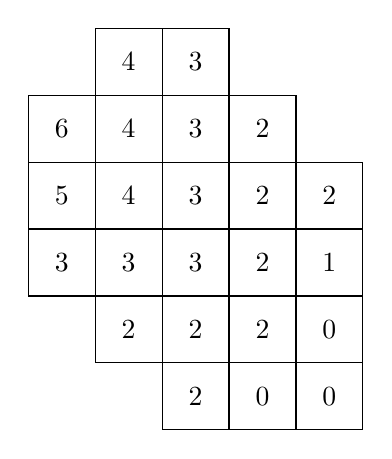
\begin{tikzpicture}[scale=0.85]
  \newcommand{\cell}[3]{% col, row, label
    \fill[white] (#1, -#2) rectangle ++(1,-1);
    \draw (#1, -#2) rectangle ++(1,-1);
    \node at (#1+0.5, -#2-0.5) {$#3$};
  }
  % Row 0 (top): cols 1-2
  \cell{1}{0}{4}  \cell{2}{0}{3}
  % Row 1: cols 0-3
  \cell{0}{1}{6}  \cell{1}{1}{4}  \cell{2}{1}{3}  \cell{3}{1}{2}
  % Row 2: cols 0-4
  \cell{0}{2}{5}  \cell{1}{2}{4}  \cell{2}{2}{3}  \cell{3}{2}{2}  \cell{4}{2}{2}
  % Row 3: cols 0-4
  \cell{0}{3}{3}  \cell{1}{3}{3}  \cell{2}{3}{3}  \cell{3}{3}{2}  \cell{4}{3}{1}
  % Row 4: cols 1-4
  \cell{1}{4}{2}  \cell{2}{4}{2}  \cell{3}{4}{2}  \cell{4}{4}{0}
  % Row 5: cols 2-4
  \cell{2}{5}{2}  \cell{3}{5}{0}  \cell{4}{5}{0}
\end{tikzpicture}
\end{center}

\item \textbf{Stacked cubes (3D).}
  A cell with label~$k$ represents $k$ unit cubes stacked
  vertically.  The result is a ``cylindric pile of cubes''
  analogous to the box-stacking picture for ordinary plane
  partitions~\cite{borodin-2007}.

\begin{center}
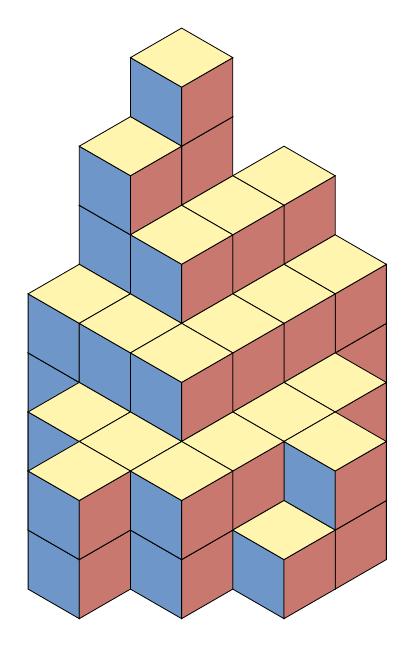
\begin{tikzpicture}[
  x={(0.65cm, -0.375cm)},
  y={(-0.65cm, -0.375cm)},
  z={(0cm, 0.75cm)}
]
\definecolor{cTop}{RGB}{255,245,175}
\definecolor{cLeft}{RGB}{110,150,200}
\definecolor{cRight}{RGB}{200,120,110}

\newcommand{\isocube}[3]{%
  \fill[cLeft, draw=black, line width=0.3pt]
    (#1,#2+1,#3) -- (#1+1,#2+1,#3) -- (#1+1,#2+1,#3+1) -- (#1,#2+1,#3+1) -- cycle;
  \fill[cRight, draw=black, line width=0.3pt]
    (#1+1,#2,#3) -- (#1+1,#2+1,#3) -- (#1+1,#2+1,#3+1) -- (#1+1,#2,#3+1) -- cycle;
  \fill[cTop, draw=black, line width=0.3pt]
    (#1,#2,#3+1) -- (#1+1,#2,#3+1) -- (#1+1,#2+1,#3+1) -- (#1,#2+1,#3+1) -- cycle;
}

\foreach \c/\r/\h in {%
  1/0/4, 0/1/6,%
  2/0/3, 1/1/4, 0/2/5,%
  2/1/3, 1/2/4, 0/3/3,%
  3/1/2, 2/2/3, 1/3/3,%
  3/2/2, 2/3/3, 1/4/2,%
  4/2/2, 3/3/2, 2/4/2,%
  4/3/1, 3/4/2, 2/5/2%
}{%
  \pgfmathtruncatemacro{\maxz}{\h-1}%
  \foreach \z in {0,...,\maxz}{%
    \isocube{\c}{\r}{\z}%
  }%
}
\end{tikzpicture}
\end{center}

\end{enumerate}
\end{remark}

\begin{remark}[Rank-3 specialisation]\label{rem:rank3}
The present research focuses on profiles relevant to the
\emph{$A_2$ Andrews--Gordon identities}.  These are parametrised
by a triple $c = (c_0, c_1, c_2)$ with $d = c_0+c_1+c_2$.
The profile string has length $T = d$ and encodes the cyclic
interlacing pattern among three partitions
$\nu^{(1)}, \nu^{(2)}, \nu^{(3)}$.
\end{remark}

The two-variable generating function is
\begin{equation}\label{eq:GK}
  \GK_c(z,q) = \sum_{\mathfrak{c} \in \CPP(c)} z^{n(\mathfrak{c})} q^{|\mathfrak{c}|}
  = \sum_{n \geq 0} g_n(q)\, z^n.
\end{equation}
Setting $z = 1$ recovers Borodin's product formula
(Section~\ref{sec:borodin}).

\subsection{The NILP model}
\label{sec:nilp}

A CPP $\mathfrak{c}$ with max entry~$n$ corresponds to
$n$ \emph{non-intersecting lattice paths} (NILPs) on the cylinder,
sandwiched between two fixed boundary paths.
The $k$-th path ($k = 1, \ldots, n$) traces the level set
$\{\text{cells with label} \geq k\}$. These $n$ paths are
\emph{free} (determined by~$\mathfrak{c}$), while the boundary
above (the \emph{profile path}, determined by~$\pi$) and the
boundary below (the \emph{zero-level}, where all labels vanish)
are fixed.  Thus there are $n + 2$ paths in total, but only
$n$ are variable.  In short:
\[
  \textbf{max entry} = n
  \quad\Longleftrightarrow\quad
  n \text{ free non-intersecting lattice paths.}
\]


\subsection{Borodin's product formula and Schur positivity}
\label{sec:borodin}

Borodin~\cite{borodin-2007} proved a cylindric analog of the
hook-product formula:
\begin{equation}\label{eq:borodin}
  \GK_c(1,q) = \prod_{s \in \widehat{\lambda}(\pi)} \frac{1}{1 - q^{h_{\widehat{\lambda}}(s)}},
\end{equation}
where $\widehat{\lambda}(\pi)$ is the cylindric diagram with
profile~$\pi$ and $h_{\widehat{\lambda}}(s) = j - i + kT$ is the
\emph{cylindric hook length} of the cell with cylindric inversion
coordinates $(i,j,k)$ (see \texttt{tex/definitions.tex}).

This generalises Stanley's hook-product formula for reverse plane
partitions~\cite{stanley-1972}:
$\sum_{\mathfrak{c} \in \RPP(\lambda)} q^{|\mathfrak{c}|}
= \prod_{s \in \lambda} 1/(1 - q^{h_\lambda(s)})$.
In the cylindric case, the hooks ``wrap around'' the cylinder,
and an additional factor $\prod_{n \geq 1} 1/(1 - q^{nT})$
(counting the base partition~$\gamma$) appears.

% 2026-02-16: Expanded with trace formula and Schur coefficient structure
\subsection{The trace formula and Schur expansion}
\label{sec:trace}

Let $\pi = (\pi_0, \ldots, \pi_{T-1})$ be the binary profile string
($T = |\pi|$), and define the Pieri operators
$G^0(u) = \Omega[Xu]$ (adds horizontal strips),
$G^1(u) = \Omega^*[Xu]$ (removes horizontal strips),
and the degree operator $D_w S_\lambda = w^{|\lambda|} S_\lambda$.
The GK generating function is a \emph{trace} over the Schur
basis~\cite{langer-thesis}:
\begin{equation}\label{eq:trace}
  \GK_c = \sum_\mu \langle S_\mu \,|\,
  G^{\pi_0}(u_0)\, G^{\pi_1}(u_1) \cdots G^{\pi_{T-1}}(u_{T-1})\,
  D_w \,|\, S_\mu \rangle,
\end{equation}
where $u_k, w$ are monomials in the refined variables
$z_0, \ldots, z_{T-1}$.
Inserting resolutions of the identity $\sum_\lambda
|S_\lambda\rangle \langle S_\lambda|$ between each operator
yields a sum over cyclic chains of partitions
$\lambda^{(0)}, \ldots, \lambda^{(T-1)}$ with
$\lambda^{(T)} = \lambda^{(0)}$, where each term is a product
of skew Schur functions:
\[
  \prod_{k=0}^{T-1}
  \langle S_{\lambda^{(k)}} | G^{\pi_k}(u_k) |
  S_{\lambda^{(k+1 \bmod T)}} \rangle
  = \prod_k s_{\text{skew}_k}(u_k).
\]
By the Littlewood--Richardson rule, each such product is
\textbf{Schur-positive}. The Schur coefficient
$\langle s_\kappa, \GK_c \rangle$ is thus a sum of
products of LR coefficients over all valid cyclic chains
of intermediate partitions---not a clean closed form,
but a definite combinatorial quantity.

\begin{question}\label{q:schur-coeffs-natural}
Give a direct combinatorial description of the Schur coefficients
$\langle s_\kappa, \GK_c \rangle$ that does not go through
iterated LR sums over cyclic chains.
\end{question}

\noindent
\textbf{Partial answer.}
The crossing-path model (Section~\ref{sec:crossing-paths})
reformulates $\langle s_\kappa, \GK_c \rangle$ as a single
count of crossing-path configurations on the cylinder
(Proposition~\ref{prop:crossing-schur}), eliminating the
intermediate partitions.  Defining statistics on these
configurations is the next step.

% 2026-02-16: Formalized cylindric Schur function definition (Korff, Postnikov, McNamara)
\begin{definition}[Cylindric skew diagram]\label{def:cyl-diagram}
Let $\lambda, \mu \in A^+_{k,n}$ (partitions with at most $k$ parts,
each $\leq n$).  For $d \geq 0$, the \emph{$(n,k)$-restricted
cylindric skew diagram of degree~$d$} is the infinite set of
lattice cells
\[
  \lambda/d/\mu
  \;:=\; \bigl\{\, (i,j) \in \Z^2 :
    \lambda[d]_i \geq j > \mu[0]_i \,\bigr\},
\]
where $\lambda[d]$ denotes the bi-infinite \emph{cylindric loop}
obtained by shifting the outline of~$\lambda$ by the period vector
$\Omega = (k, -n)$, then translating by $(d,0)$.
Concretely, $\lambda[d]$ has a fundamental region with parts
$(n^d, \lambda_1, \ldots, \lambda_k)$.  The diagram is
$\Omega$-periodic: translating by $(k, -n)$ maps it to itself.
For $d = 0$, this recovers the ordinary skew diagram $\lambda/\mu$.
\end{definition}

COULD YOU DRAW ME A DIAGRAM HERE. I DON"T GET IT

\begin{definition}[Cylindric Schur function]\label{def:cyl-schur}
A \emph{semistandard cylindric tableau} of shape $\lambda/d/\mu$
is a map $T : \lambda/d/\mu \to \N$ satisfying:
\begin{enumerate}
\item \textbf{Periodicity:}
  $T(i,j) = T(i+k,\, j-n)$ for all $(i,j) \in \lambda/d/\mu$;
\item \textbf{Weak row increase:}
  $T(i,j) \leq T(i,j+1)$ when $(i,j+1) \in \lambda/d/\mu$;
\item \textbf{Strict column increase:}
  $T(i,j) < T(i+1,j)$ when $(i+1,j) \in \lambda/d/\mu$.
\end{enumerate}
The weight $\mathbf{x}^T = \prod_i x_{T(i,j)}$ is taken over one
fundamental period ($k+d$ consecutive rows).
The \emph{cylindric Schur function} is
\[
  s_{\lambda/d/\mu}(x_1, x_2, \ldots)
  = \sum_T \mathbf{x}^T,
\]
summed over all semistandard cylindric tableaux~$T$ of shape
$\lambda/d/\mu$.  This is a symmetric function
(McNamara~\cite{mcnamara-2006}; see also Korff~\cite{korff-2011},
Postnikov~\cite{postnikov-2005}).
\end{definition}

% 2026-02-17: Answered — yes, they are the same object viewed differently
\begin{remark}
A semistandard cylindric tableau of shape $\lambda/d/\mu$ is
the same object as a CPP with the corresponding profile~$\pi$.
Given a CPP $(\mu^0, \ldots, \mu^T)$, label each cell of the
horizontal strip $\mu^k \setminus \mu^{k-1}$ (when $\pi_k = 1$)
with entry~$k$; the result is a semistandard cylindric tableau.
Conversely, reading the entry sets of a cylindric tableau by
value recovers the partition sequence.
The profile~$\pi$ determines the cylindric shape
(see Definition~\ref{def:cyl-diagram}).
\end{remark}

\begin{remark}
% 2026-02-16
This Schur positivity of $\GK_c$ should be distinguished from
the question of whether individual cylindric Schur functions
$s_{\lambda/d/\mu}$ are Schur-positive. McNamara~\cite{mcnamara-2006}
showed that cylindric Schur functions can have
\textbf{negative} Schur coefficients.
The full generating function $\GK_c$, being a sum over all
cylindric shapes, is positive by the trace/LR argument above,
even though individual summands need not be.
\end{remark}

\subsection{Local rules: motivation from the Cauchy identity}
\label{sec:local-rules}

% 2026-02-16: Rewritten with Cauchy identity motivation from thesis (chap3.tex)
The \emph{local rule} is the combinatorial engine behind the
growth-diagram proof of Borodin's identity.
Its existence is motivated by the \textbf{Cauchy identity}:
\[
  \sum_\lambda S_\lambda[X_n]\, S_\lambda[Y_n]
  = \prod_{i,j=1}^n \frac{1}{1 - x_i y_j}.
\]

THERE IS MORE DETAIL IN DEFINITIONS.TEX INCLUDE IT

An inductive proof (adding one variable at a time) reduces this
to matching coefficients of $S_\alpha[X_{n-1}]\, S_\beta[Y_{n-1}]$
on both sides.  On the RHS, after factoring out
$1/(1 - x_n y_n)$, one sums over pairs $(m, \mu)$ with
$\mu \in D(\alpha) \cap D(\beta)$ and $m \geq 0$; on the LHS,
one sums over $\lambda \in U(\alpha) \cap U(\beta)$.
The identity holds if and only if there exists a
weight-preserving bijection between these two sets.

\begin{definition}[Local rule]\label{def:local-rule}
Let $D(\alpha)$ be the set of partitions obtained from $\alpha$
by removing a horizontal strip, and $U(\alpha)$ the set obtained
by adding one.
A \emph{local rule} is a bijection
\[
  \mathfrak{U}_{\alpha,\beta} :
  \bigl(\Z_{\geq 0} \times (D(\alpha) \cap D(\beta))\bigr)
  \xrightarrow{\;\sim\;}
  U(\alpha) \cap U(\beta),
\]
satisfying $|\lambda| = m + |\alpha| + |\beta| - |\nu|$
whenever $\mathfrak{U}_{\alpha,\beta}(m, \nu) = \lambda$.
The inverse is
$\mathfrak{D}_{\alpha,\beta}(\lambda) = (m, \nu)$.
\end{definition}

There are exactly \textbf{two} natural choices of local rule
(see~\cite{langer-thesis}, Section~3.2):
\begin{enumerate}
\item \textbf{RSK rule}: corresponds to the Robinson--Schensted--Knuth
  correspondence;
\item \textbf{Burge rule}: corresponds to the Burge correspondence.
\end{enumerate}
Both satisfy the weight condition and the commutativity property
$\mathfrak{L}_i \circ \mathfrak{L}_j = \mathfrak{L}_j \circ \mathfrak{L}_i$
when $|i - j| \geq 2$, which ensures that the growth diagram
is well-defined regardless of the order in which inversions are processed.

% 2026-02-16: Added explicit Burge rule from thesis chap1.tex, Section 3.2

ALSO INCLUDE THE EXPLICIT RSK RULE

\subsubsection*{Explicit Burge rule}

We describe the \textbf{Burge local rule} explicitly
(see~\cite{langer-thesis}, Section~3.2).

\smallskip\noindent\textbf{Down operator}
$\mathfrak{D}_{\alpha,\beta}(\lambda) = (m, \mu)$:
\begin{enumerate}
\item Let $\overline{A} = \{i : \lambda'_i > \alpha'_i\}$
  and $\overline{B} = \{i : \lambda'_i > \beta'_i\}$
  (columns of $\lambda$ strictly longer than those of
  $\alpha$, $\beta$).
\item For each $i \in \overline{A} \cap \overline{B}$
  (in decreasing order), assign $\delta(i)$ to be the
  largest column index $< i$ not in
  $\overline{A} \cup \overline{B}$ and not already assigned.
  Set $\overline{C} = \{\delta(i) > 0 : i \in \overline{A} \cap \overline{B}\}$.
\item Obtain $\mu$ from $\lambda$ by removing a box from
  each column in $\overline{A} \cup \overline{B} \cup \overline{C}$.
  Set $m = \#\{\delta(i) \leq 0\}$.
\end{enumerate}

\smallskip\noindent\textbf{Up operator}
$\mathfrak{U}_{\alpha,\beta}(m, \mu) = \lambda$:
\begin{enumerate}
\item Let $A = \{i : \alpha'_i > \mu'_i\}$
  and $B = \{i : \beta'_i > \mu'_i\}$.
\item For each $i \in A \cap B$ (in increasing order),
  assign $\epsilon(i)$ to be the smallest column index
  $> i$ not in $A \cup B$ and not already assigned.
  Set $C = \{\epsilon(i)\}$.
\item Let $D$ be the first $m$ elements of
  $\Z_{>0} \setminus (A \cup B \cup C)$.
  Obtain $\lambda$ from $\mu$ by adding a box to each column
  in $A \cup B \cup C \cup D$.
\end{enumerate}

\begin{example}[Burge rule]\label{ex:burge}
Take $\alpha = (6,5,5,3)$, $\beta = (6,6,5,2)$,
$\lambda = (7,6,5,3,1)$.  Then:
\begin{align*}
  \lambda' &= (5,4,4,3,3,2,1), \quad
  \overline{A} = \{1,6,7\}, \quad
  \overline{B} = \{1,3,7\}. \\
  \overline{A} \cap \overline{B} &= \{1,7\}.
\end{align*}
Processing $i = 7$: $\delta(7) = 5$ (largest $< 7$
not in $\{1,3,6,7\}$).
Processing $i = 1$: $\delta(1) = 0$ (no column $< 1$ is available).
So $\overline{C} = \{5\}$, $m = 1$, and $\mu$ is obtained by
removing a box from columns $\{1,3,5,6,7\}$, giving
$\mu = (6,5,4,2)$.
\[
  \boxed{\mathfrak{D}_{(6,5,5,3),(6,6,5,2)}(7,6,5,3,1)
  = \bigl(1,\,(6,5,4,2)\bigr).}
\]
The inverse $\mathfrak{U}_{\alpha,\beta}(1,(6,5,4,2))
= (7,6,5,3,1)$ follows by the dual greedy matching.
\end{example}

\subsection{The cylindric growth diagram}
\label{sec:growth-diagram}

A \emph{cylindric growth diagram} with profile~$\pi$ is a
labelling of the cylindric poset (the quotient
$\Z^2 / (x,y) \sim (x+n, y-m)$) by integer partitions at
vertices and nonneg integers at faces, such that:
\begin{enumerate}
\item adjacent partitions along edges differ by a horizontal strip;
\item all sufficiently deep vertices carry the same label~$\gamma$;
\item the local rule $\mathfrak{U}_{\alpha,\beta}(m,\nu) = \lambda$
  holds at every face.
\end{enumerate}
The upper boundary reads off a CPP
$\mathfrak{c} \in \CPP(\pi)$; the face labels assemble into an
arbitrarily labelled cylindric diagram $\mathfrak{d} \in \mathrm{ALCD}(\pi)$.
By the invertibility of the local rule, this gives a
\emph{strongly weight-preserving} bijection~\cite{langer-thesis}:
\begin{equation}\label{eq:growth-bijection}
  \psi_\pi : (\mathrm{IP}, \mathrm{ALCD}(\pi))
  \xrightarrow{\;\sim\;} \CPP(\pi),
\end{equation}
satisfying
$|\mu^k| = |\gamma| + |\mathrm{diag}(k)|_{\mathfrak{d}}$
for each step $k$.

This proves Borodin's identity: CPPs biject with
(partition~$\gamma$, labelled cylindric diagram~$\mathfrak{d}$),
and the hook-product formula counts the latter.
The growth diagram mirrors the algebraic proof step-by-step:
each row corresponds to one Pieri operator in the trace
formula~\eqref{eq:trace}, and the vertex labels are the
intermediate partitions.

% 2026-02-16: Growth diagram TikZ from definitions.tex
\begin{example}[Growth diagram]\label{ex:growth-diagram}
Below is a growth diagram for profile $\pi = 00101$
(i.e.\ $c = (2,1,2)$, $d = 5$).
Vertex labels are partitions; face labels are nonneg
integers consumed by the local rule.
The bottom row repeats the base partition $\gamma = (3,2)$
(periodically on the cylinder); the top vertex gives
the CPP entries.

\begin{center}
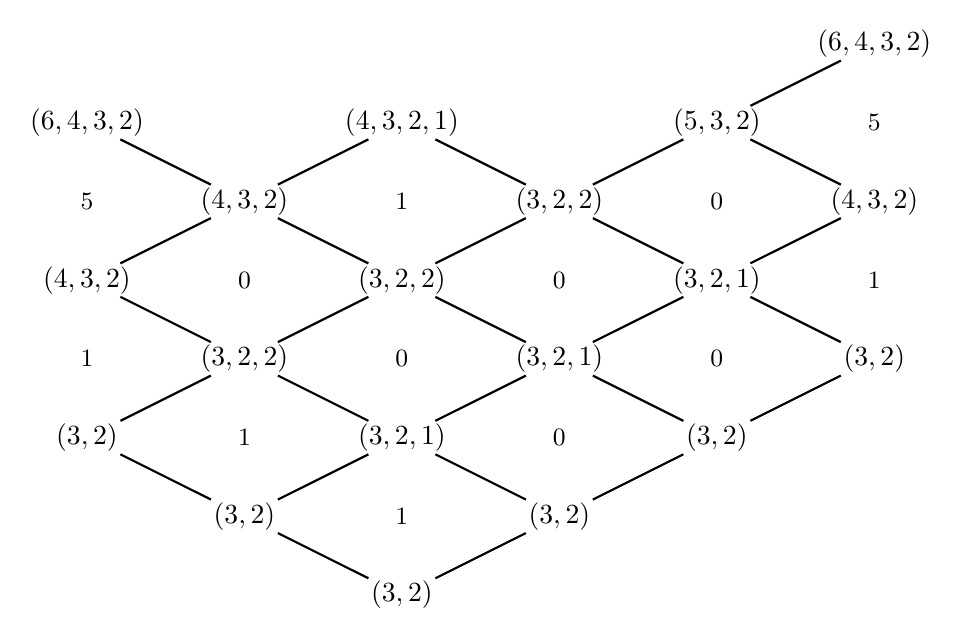
\begin{tikzpicture}[scale=1]

\path (-4,2) node[inner sep=0.3mm](A0){$(3,2)$};
\path (-2,1) node[inner sep=0.3mm](B0){$(3,2)$};
\path (0,0) node[inner sep=0.3mm](C0){$(3,2)$};
\path (2,1) node[inner sep=0.3mm](D0){$(3,2)$};
\path (4,2) node[inner sep=0.3mm](E0){$(3,2)$};
\path (6,3) node[inner sep=0.3mm](F0){$(3,2)$};

\path (-4,4) node[inner sep=0.3mm](A1){$(4,3,2)$};
\path (-2,3) node[inner sep=0.3mm](B1){$(3,2,2)$};
\path (0,2) node[inner sep=0.3mm](C1){$(3,2,1)$};
\path (2,3) node[inner sep=0.3mm](D1){$(3,2,1)$};
\path (4,4) node[inner sep=0.3mm](E1){$(3,2,1)$};
\path (6,5) node[inner sep=0.3mm](F1){$(4,3,2)$};

\path (-4,6) node[inner sep=0.3mm](A2){$(6,4,3,2)$};
\path (-2,5) node[inner sep=0.3mm](B2){$(4,3,2)$};
\path (0,4) node[inner sep=0.3mm](C2){$(3,2,2)$};
\path (2,5) node[inner sep=0.3mm](D2){$(3,2,2)$};
\path (4,6) node[inner sep=0.3mm](E2){$(5,3,2)$};
\path (6,7) node[inner sep=0.3mm](F2){$(6,4,3,2)$};

\path (0,6) node[inner sep=0.3mm](C3){$(4,3,2,1)$};

\draw[thick] (A0) -- (B0) -- (C0) -- (D0) -- (E0) -- (F0);
\draw[thick] (A1) -- (B1) -- (C1) -- (D1) -- (E1) -- (F1);
\draw[thick] (A2) -- (B2) -- (C2) -- (D2) -- (E2) -- (F2);

\draw[thick] (A1) -- (B2) -- (C3);
\draw[thick] (A0) -- (B1) -- (C2);
\draw[thick] (B0) -- (C1);
\draw[thick] (D0) -- (C1);
\draw[thick] (E0) -- (D1) -- (C2);
\draw[thick] (F0) -- (E1) -- (D2) -- (C3);
\draw[thick] (F1) -- (E2);

% Face labels (integers at each face)
\path (-4,3) node[inner sep=0.3mm]{\small $1$};
\path (-2,2) node[inner sep=0.3mm]{\small $1$};
\path (0,1) node[inner sep=0.3mm]{\small $1$};
\path (2,2) node[inner sep=0.3mm]{\small $0$};
\path (4,3) node[inner sep=0.3mm]{\small $0$};
\path (6,4) node[inner sep=0.3mm]{\small $1$};

\path (-4,5) node[inner sep=0.3mm]{\small $5$};
\path (-2,4) node[inner sep=0.3mm]{\small $0$};
\path (0,3) node[inner sep=0.3mm]{\small $0$};
\path (2,4) node[inner sep=0.3mm]{\small $0$};
\path (4,5) node[inner sep=0.3mm]{\small $0$};
\path (6,6) node[inner sep=0.3mm]{\small $5$};

\path (0,5) node[inner sep=0.3mm]{\small $1$};

\end{tikzpicture}
\end{center}
The face labels on each row encode the CPP entries at
that level.  The left and right ends of each row are
identified on the cylinder.
\end{example}

\begin{remark}[Two bijections and Sch\"utzenberger]\label{rem:two-bijections}
The RSK and Burge choices yield bijections $\psi_R, \psi_B$.
Their composition
$\psi_R \circ \psi_B^{-1} : \CPP(\pi) \to \CPP(\pi)$
is a \emph{Sch\"utzenberger-type involution} on CPPs,
preserving the profile and the weight.
Its representation-theoretic meaning at the level of
Tingley's $\widehat{\mathfrak{sl}}_n$
crystal~\cite{tingley-2007} is an open question.
\end{remark}


%% ================================================================
\part{Cool Concepts}
\label{part:concepts}
%% ================================================================

%% ==================================================================
\section{Quasi-symmetric functions and $L$-positivity}
\label{sec:qsym}
%% ==================================================================

\subsection{The frequency generating function}

For a CPP $\pi$, define the value frequency
$\#_k(\pi) = |\{(i,j) : \nu^{(i)}_j = k\}|$.
The \emph{frequency generating function} is
\begin{equation}\label{eq:GKtilde}
  \widetilde{\GK}_c(\mathbf{z})
  = \sum_{\pi \in \CPP(c)}
  z_1^{\#_1(\pi)} z_2^{\#_2(\pi)} \cdots
  \in \Z[[z_1, z_2, \ldots]].
\end{equation}
Under $z_k \mapsto q^k$, this recovers $\GK_c(1,q)$.

\begin{observation}[Verified: 55 profiles, $d \leq 5$]
\label{obs:qsym}
$\widetilde{\GK}_c$ is quasi-symmetric:
$\widetilde{\GK}_c = \sum_\alpha a_\alpha(c)\, M_\alpha$
with $a_\alpha \in \Z_{\geq 0}$.
It is \emph{not} symmetric ($a_{(2,1)} \neq a_{(1,2)}$ in general).
\end{observation}

The quasi-symmetry follows from the observation that the
interlacing conditions~\eqref{eq:interlacing} depend only on the
\emph{relative order} of entries, not their absolute values.
This is an instance of Stanley's $P$-partition theory:

By the Stanley--Gessel theory of $P$-partitions
(Section~\ref{sec:P-partitions}), the generating function
of any labeled poset is quasi-symmetric and $L$-positive
(Theorem~\ref{thm:P-part-qsym-full}).
The CPP interlacing conditions are precisely of
$P$-partition type (weak and strict comparisons on entries),
and hence $\widetilde{\GK}_c$ is quasi-symmetric.

\subsection{$L$-positivity}

% 2026-02-16: Clarified open problem status and symmetrisation
\begin{remark}[$L$-positivity as open problem]\label{rem:L-pos-open}
While $L$-positivity of $\widetilde{\GK}_c$ is computationally
verified, a \textbf{proof} remains open.  The $P$-partition
theorem gives $L$-positivity for any \emph{fixed} max entry
(the poset is acyclic after unrolling the cycle), but
$\widetilde{\GK}_c$ sums over \emph{all} max entries, and
it is not obvious that an infinite sum of $L$-positive
functions remains $L$-positive.
\end{remark}

\begin{remark}[Symmetrisation]\label{rem:symmetrisation}
Under the natural projection $\QSym \to \Sym$ given by
$M_\alpha \mapsto m_{\mathrm{sort}(\alpha)}$
(equivalently $L_\alpha \mapsto s_{\mathrm{sort}(\alpha)}$),
$L$-positivity implies Schur positivity.
Concretely, $\widetilde{\GK}_c$ maps to
$\sum_\alpha b_\alpha(c)\, s_{\mathrm{sort}(\alpha)}$,
grouping compositions by their underlying partition.
The symmetrisation of $\widetilde{\GK}_c$ is thus a
Schur-positive symmetric function, recovering the Schur
positivity of $\GK_c$ from a finer quasi-symmetric structure.
\end{remark}

The \emph{fundamental quasi-symmetric functions} $L_\alpha$
(also denoted $F_\alpha$) are a second basis of $\QSym$:
\[
  L_\alpha = \sum_{\beta \preceq \alpha} M_\beta,
\]
where $\beta \preceq \alpha$ means $\beta$ refines $\alpha$.
The $M$-to-$L$ conversion uses M\"obius inversion:
$b_\alpha = \sum_{\beta \succeq \alpha}
(-1)^{\ell(\beta)-\ell(\alpha)} a_\beta$.

\begin{observation}[Verified: 55 profiles, $d \leq 5$]
\label{obs:L-pos}
$\widetilde{\GK}_c$ is $L$-positive:
$\widetilde{\GK}_c = \sum_\alpha b_\alpha(c)\, L_\alpha$
with $b_\alpha \in \Z_{\geq 0}$.
\end{observation}

$L$-positivity is strictly stronger than $M$-positivity
(which is automatic since $a_\alpha$ counts CPPs).
Stabilised $L$-coefficients exhibit product structure:
$c = (1,1,0)$ gives $b_\alpha^{\mathrm{stab}} = 2^{\ell(\alpha)}$;
$c = (2,1,1)$ gives $5^{\ell(\alpha)}$.


%% ==================================================================
\section{Descent statistics: charge, cocharge, and $0$-Hecke}
\label{sec:descent}
%% ==================================================================

% 2026-02-16: Added reading words, LR rule, explicit charge reading word
\subsection{Reading words and the Littlewood--Richardson rule}
\label{sec:reading-word}

Both the Littlewood--Richardson rule and the charge statistic
depend on a \emph{reading word}: a linear ordering of the cells
of a (skew) tableau.

\begin{definition}[Reading word]\label{def:reading-word}
The \emph{reverse reading word} of a (skew) tableau~$T$ is the
sequence of entries obtained by reading each row from
\textbf{right to left}, starting from the \textbf{top row} and
proceeding downward.  (Equivalently: columns from right to left,
top to bottom within each column.)
\end{definition}

\begin{definition}[Lattice word]\label{def:lattice-word}
A word $w = w_1 w_2 \cdots w_N$ in the alphabet
$\{1, 2, \ldots, k\}$ is a \emph{lattice word}
(or \emph{ballot sequence}, or \emph{Yamanouchi word})
if for every prefix $w_1 \cdots w_j$ and every letter~$i$,
\[
  \#\{m \leq j : w_m = i\} \;\geq\; \#\{m \leq j : w_m = i{+}1\}.
\]
In words: at every point in the word, we have seen at least as
many $i$'s as $(i{+}1)$'s, for all~$i$.
\end{definition}

\begin{theorem}[Littlewood--Richardson rule]\label{thm:LR}
$s_\mu \cdot s_\nu = \sum_\lambda c^{\lambda}_{\mu\nu}\, s_\lambda$,
where the \emph{Littlewood--Richardson coefficient}
$c^{\lambda}_{\mu\nu}$ counts the number of semistandard
skew tableaux of shape $\lambda / \mu$ and content~$\nu$
whose reverse reading word is a lattice word.
\end{theorem}

\begin{example}[LR coefficients for $s_{(2,1)}^2$]
\label{ex:LR}
Compute $c^{(3,2,1)}_{(2,1),(2,1)}$: fill the skew shape
$(3,2,1)/(2,1)$ with content $(2,1) = \{1,1,2\}$.  The skew
cells are $(1,3)$, $(2,2)$, $(3,1)$ (one per row, all in
different columns, so no row/column constraints between them).
All three assignments are valid SSYT:
\[
\renewcommand{\arraystretch}{1.2}
\begin{array}{cccc}
  \text{Filling} & (1,3),(2,2),(3,1) & \text{Rev.\ reading word} & \text{Lattice?} \\
  \hline
  T_1 & 1,\; 1,\; 2 & 1,\;1,\;2 & \text{\textbf{Yes}} \\
  T_2 & 1,\; 2,\; 1 & 1,\;2,\;1 & \text{\textbf{Yes}} \\
  T_3 & 2,\; 1,\; 1 & 2,\;1,\;1 & \text{No: prefix ``$2$'' has $\#_2 > \#_1$}
\end{array}
\]
$T_3$ fails at the very first letter: the prefix ``$2$''
has one~$2$ but zero~$1$'s.  Thus
$c^{(3,2,1)}_{(2,1),(2,1)} = 2$.

\smallskip\noindent
\textbf{Key point.}  The reading word turns a 2D object
(a skew tableau) into a 1D word.  The lattice condition
selects which fillings ``count.''  The same idea---choose
a reading order, then check a combinatorial property of
the resulting word---is what we seek for CPPs.
\end{example}

\subsection{Charge, cocharge, and Kostka--Foulkes polynomials}

\begin{definition}[Kostka--Foulkes polynomial]\label{def:KF}
Let $\lambda \vdash n$ and $\mu \vdash n$.
The \emph{Kostka--Foulkes polynomial} $K_{\lambda,\mu}(q)$ is the
transition coefficient between the Schur basis and the
Hall--Littlewood basis:
$s_\lambda = \sum_\mu K_{\lambda,\mu}(q)\, P_\mu(x;q)$.
Equivalently, $K_{\lambda,\mu}(q)$ is the coefficient of
$s_\lambda$ in $\sum_T q^{\charge(T)}$, summed over all
$T \in \SSYT(\lambda, \mu)$.
\end{definition}

\begin{definition}[Charge statistic]\label{def:charge}
The \emph{charge} of Lascoux--Sch\"utzen\-ber\-ger~\cite{LS78}
is a statistic $\charge : \SSYT(\lambda, \mu) \to \Z_{\geq 0}$
defined as follows.  Given a semistandard tableau~$T$ of
shape~$\lambda$ and content~$\mu$:
\begin{enumerate}
\item Form the \emph{reading word} of~$T$: read each row
  from \textbf{left to right}, starting from the \textbf{bottom
  row} and proceeding upward.
  (For a standard tableau this gives a permutation;
  for a semistandard tableau, a word with repeated letters.)
\item Decompose the reading word into \emph{standard subwords}
  (each containing exactly one copy of each letter $1, \ldots, k$).
\item For each standard subword $\sigma$ (a permutation of
  $\{1,\ldots,k\}$), define $\operatorname{index}(1) = 0$
  and, for $i = 2, \ldots, k$:
  \[
    \operatorname{index}(i) =
    \begin{cases}
      \operatorname{index}(i{-}1) & \text{if letter $i$ appears
        to the \emph{right} of letter $i{-}1$ in $\sigma$,} \\
      \operatorname{index}(i{-}1) + 1 & \text{otherwise.}
    \end{cases}
  \]
  Set $\charge(\sigma) = \sum_{i=1}^{k} \operatorname{index}(i)$.
\item The charge of~$T$ is the sum of charges of its
  standard subwords.
\end{enumerate}
The \emph{cocharge} is $\cocharge(T) = n(\lambda,\mu) - \charge(T)$,
where $n(\lambda,\mu) = \sum_{i < j} \min(\mu_i, \lambda'_j)$.
\end{definition}

% 2026-02-16: Worked charge example
\begin{example}[Computing charge]\label{ex:charge}
Take $\lambda = (2,1)$, $\mu = (1,1,1)$.
Since $\mu = 1^3$, each SSYT is a standard Young tableau.
There are two:
\[
  T_1 = \begin{array}{|c|c|}\hline 1 & 2 \\\hline 3 \\\cline{1-1}\end{array}
  \qquad\qquad
  T_2 = \begin{array}{|c|c|}\hline 1 & 3 \\\hline 2 \\\cline{1-1}\end{array}
\]
Reading words (bottom to top, left to right):
$w(T_1) = 3\,1\,2$ and $w(T_2) = 2\,1\,3$.

\smallskip\noindent
\textbf{Charge of $T_1$} ($\sigma = 3\,1\,2$):
\begin{itemize}
\item $\operatorname{index}(1) = 0$.
\item Letter $2$ is at position~3, letter $1$ at position~2:
  $2$ is to the \emph{right} of $1$ $\Rightarrow$
  $\operatorname{index}(2) = 0$.
\item Letter $3$ is at position~1, letter $2$ at position~3:
  $3$ is to the \emph{left} of $2$ $\Rightarrow$
  $\operatorname{index}(3) = 0 + 1 = 1$.
\end{itemize}
$\charge(T_1) = 0 + 0 + 1 = 1$.

\smallskip\noindent
\textbf{Charge of $T_2$} ($\sigma = 2\,1\,3$):
\begin{itemize}
\item $\operatorname{index}(1) = 0$.
\item Letter $2$ at position~1, letter $1$ at position~2:
  $2$ is to the \emph{left} of $1$ $\Rightarrow$
  $\operatorname{index}(2) = 1$.
\item Letter $3$ at position~3, letter $2$ at position~1:
  $3$ is to the \emph{right} of $2$ $\Rightarrow$
  $\operatorname{index}(3) = 1$.
\end{itemize}
$\charge(T_2) = 0 + 1 + 1 = 2$.

\smallskip
Therefore $K_{(2,1),(1^3)}(q) = q^1 + q^2 = q + q^2$.
\end{example}

The key theorem is:
\[
  K_{\lambda,\mu}(q) = \sum_{T \in \SSYT(\lambda,\mu)} q^{\charge(T)}
  \in \N[q].
\]
The nonnegativity is highly nontrivial (proved via the theory
of crystal bases, or equivalently via Haiman's proof using
the $n!$-conjecture).

We verified computationally that $Q_{n,c}(q)$ does \emph{not}
decompose as a nonneg sum of Kostka--Foulkes polynomials.
However, the $L$-positivity of $\widetilde{\GK}_c$ suggests
a \emph{different} charge-like statistic may exist on CPPs,
one adapted to compositions rather than partitions.
See \texttt{scripts/analyze\_Q.py}.

\begin{question}\label{q:charge-statistic}
Does there exist a charge-like statistic on CPPs
(or on $(S,U,\nu)$ triples) that explains the positivity
of $Q_{n,c}(q)$?
\end{question}

\begin{question}\label{q:qt-analog}
Is there a $(q,t)$-analog of the conjecture?
The Hall--Littlewood case ($t = 0$ in the Macdonald framework)
should recover the original conjecture.  Replacing the Schur
basis by the Macdonald basis $\{P_\lambda(x;q,t)\}$ in the trace
formula gives a $(q,t)$-weighted GK function
(Section~\ref{sec:macdonald}); does the
$Q$-polynomial extraction yield a polynomial with
nonneg coefficients in $q$ and $t$?

\textbf{Partial answer} (Section~\ref{sec:mac-schur-rational}):
The $P/Q$-basis formulation gives \emph{rational functions}
of $q,t$, not polynomials, so the question is ill-posed
in that basis. The modified Macdonald basis $\tilde{H}_\mu$
does give polynomial Schur coefficients (Haiman), but
reformulating the Borodin identity in $\tilde{H}$ is open.
\end{question}

\subsection{$0$-Hecke modules}

% 2026-02-16: Expanded with references and context
The \emph{$0$-Hecke algebra} $H_n(0)$ is the quotient of the free
algebra on generators $T_1, \ldots, T_{n-1}$ by the Coxeter braid
relations and the idempotent relations $T_i^2 = T_i$.
Its irreducible modules are one-dimensional and indexed by
compositions of~$n$.

By the work of Tewari--van~Willigenburg~\cite{tewari-vanwilligenburg},
$L$-positivity of a quasi-symmetric function $f$ is equivalent to
$f$ being the \emph{quasi-symmetric characteristic} of an
$H_n(0)$-module. Thus:

\begin{corollary}
Observation~\ref{obs:L-pos} implies the existence of a graded
$H_n(0)$-module $M_c$ such that
$\operatorname{ch}(M_c) = \widetilde{\GK}_c$.
\end{corollary}

\begin{conjecture}\label{conj:descent}
There exists a natural descent-type statistic $\alpha(\pi)$ on
CPPs such that
$\widetilde{\GK}_c = \sum_\pi L_{\alpha(\pi)}$.
\end{conjecture}

Finding such a statistic would give a combinatorial proof of
$L$-positivity and could illuminate the original conjecture.


%% ==================================================================
\section{$P$-partitions}
\label{sec:P-partitions}
%% ==================================================================

% 2026-02-16: Full pedagogical treatment of P-partitions with examples.
% Key references:
% - Stanley, Ordered structures and partitions (1972)
% - Gessel, Multipartite P-partitions (1984)
% - Gessel--Reutenauer (1993) for the connection to QSym
% - McNamara (2006) for cylindric generalisation

\subsection{What is a $P$-partition?}

A $P$-partition is a generalisation of a semistandard Young
tableau.  The idea: instead of filling the cells of a Young
diagram, you fill the elements of a \emph{poset} with positive
integers, subject to ordering rules.

\begin{definition}[Labeled poset]\label{def:labeled-poset}
A \emph{labeled poset} is a pair $(P, \omega)$ where:
\begin{itemize}
\item $P$ is a finite partially ordered set (poset), and
\item $\omega : P \to \{1, 2, \ldots, |P|\}$ is a bijection
  (a labeling of the elements by distinct integers).
\end{itemize}
A \emph{descent} of $(P,\omega)$ is a covering relation
$x \lessdot_P y$ where $\omega(x) > \omega(y)$
(the label goes \emph{down} while the poset goes \emph{up}).
An \emph{ascent} is one where $\omega(x) < \omega(y)$.
\end{definition}

\begin{definition}[$(P,\omega)$-partition]\label{def:P-partition}
Given a labeled poset $(P,\omega)$, a \emph{$(P,\omega)$-partition}
is a map $\sigma : P \to \Z_{> 0}$ such that for every
covering relation $x \lessdot_P y$:
\begin{itemize}
\item \textbf{At an ascent}
  ($\omega(x) < \omega(y)$):
  require $\sigma(x) \leq \sigma(y)$ \quad (weakly increasing),
\item \textbf{At a descent}
  ($\omega(x) > \omega(y)$):
  require $\sigma(x) < \sigma(y)$ \quad (strictly increasing).
\end{itemize}
\end{definition}

\noindent
\textbf{In plain language:}  the poset $P$ tells you which
elements must be compared.  The labeling $\omega$ tells you
whether each comparison is weak~($\leq$) or strict~($<$).

\begin{example}[SSYT as a $P$-partition]\label{ex:ssyt-as-P}
A semistandard Young tableau of shape $\lambda = (2,2)$ is a
filling of four cells with positive integers, rows weakly
increasing left to right, columns strictly increasing bottom
to top (French convention).  This is a $P$-partition where:

\smallskip
The poset $P$ has four elements arranged in a $2 \times 2$ grid,
with covering relations
$(1,1) \lessdot (1,2)$ (same row),
$(2,1) \lessdot (2,2)$ (same row),
$(1,1) \lessdot (2,1)$ (same column),
$(1,2) \lessdot (2,2)$ (same column).
The labeling $\omega$ is chosen so that:
\begin{itemize}
\item Row neighbours are ascents ($\omega$ increases left to right)
  $\Rightarrow$ weak inequality~$\leq$,
\item Column neighbours are descents ($\omega$ decreases bottom
  to top) $\Rightarrow$ strict inequality~$<$.
\end{itemize}
For instance:
$\omega(1,1) = 2$, $\omega(1,2) = 4$,
$\omega(2,1) = 1$, $\omega(2,2) = 3$.
Then $(1,1) \lessdot (1,2)$: $\omega = 2 < 4$ (ascent $\Rightarrow \leq$, rows weakly increasing).
And $(1,1) \lessdot (2,1)$: $\omega = 2 > 1$ (descent $\Rightarrow <$, columns strictly increasing).
\end{example}

\begin{example}[A non-tableau $P$-partition]\label{ex:non-tableau-P}
Consider a poset $P$ on three elements $\{a, b, c\}$ with
a single relation $a <_P b$ (so $c$ is incomparable to both).
Label: $\omega(a) = 2$, $\omega(b) = 1$, $\omega(c) = 3$.

Since $\omega(a) = 2 > 1 = \omega(b)$ and $a \lessdot_P b$,
this is a \emph{descent}, so any $(P,\omega)$-partition must
have $\sigma(a) < \sigma(b)$ (strict).  The value $\sigma(c)$
is unconstrained (since $c$ is incomparable to everything).

Some valid $(P,\omega)$-partitions:
$(\sigma(a), \sigma(b), \sigma(c)) = (1, 2, 1)$,\;
$(1, 3, 5)$,\; $(2, 4, 1)$.

\noindent
But $(3, 3, 1)$ is \textbf{not} valid because
$\sigma(a) = 3 \not< 3 = \sigma(b)$.
\end{example}

\subsection{The generating function and $L$-positivity}
\label{sec:P-part-gf}

Given a labeled poset $(P,\omega)$, define its
\emph{$P$-partition generating function}:
\[
  \Gamma_{(P,\omega)}(\mathbf{z})
  = \sum_\sigma \prod_{p \in P} z_{\sigma(p)},
\]
where the sum is over all $(P,\omega)$-partitions
$\sigma : P \to \Z_{>0}$.

\begin{example}[Generating function of Example~\ref{ex:non-tableau-P}]
\label{ex:P-gf}
For $P = \{a, b, c\}$ with $a <_P b$ (descent) and
$c$ incomparable:
\[
  \Gamma_{(P,\omega)}
  = \sum_{\substack{i < j \\ k \geq 1}} z_i\, z_j\, z_k
  = \Bigl(\sum_{i < j} z_i z_j\Bigr)
    \Bigl(\sum_{k \geq 1} z_k\Bigr).
\]
This is quasi-symmetric: if we set $z_1 = z_2 = \cdots = z_n = 1$
and all others to $0$, the result depends only on~$n$
(it equals $\binom{n}{2} \cdot n$), not on \emph{which}~$n$
variables we chose.
\end{example}

The fundamental theorem is:

\begin{theorem}[Stanley 1972, Gessel 1984]
\label{thm:P-part-qsym-full}
For any labeled poset $(P,\omega)$:
\begin{enumerate}
\item $\Gamma_{(P,\omega)}$ is quasi-symmetric.
\item $\Gamma_{(P,\omega)}$ is $L$-positive:
  $\Gamma_{(P,\omega)} = \sum_\alpha b_\alpha L_\alpha$
  with $b_\alpha \in \Z_{\geq 0}$.
\item The coefficient $b_\alpha$ counts the number of
  \emph{linear extensions} of~$P$ whose \emph{descent
  composition} equals~$\alpha$.
\end{enumerate}
\end{theorem}

The key notion is:

\begin{definition}[Linear extension and descent composition]
\label{def:linear-ext}
A \emph{linear extension} of a poset~$P$ on elements
$\{p_1, \ldots, p_n\}$
is a listing $\pi = \pi_1, \pi_2, \ldots, \pi_n$ of the
elements of~$P$ such that if $x <_P y$ then $x$ appears
before~$y$ in~$\pi$.  (It is a ``reading word'': a way to read
all elements of~$P$ in an order compatible with the
partial order.)

The \emph{descent set} of a linear extension $\pi$ (with
respect to the labeling $\omega$) is
\[
  \Des(\pi) = \{i : \omega(\pi_i) > \omega(\pi_{i+1})\}
  \subseteq \{1, 2, \ldots, n{-}1\}.
\]
The \emph{descent composition} is the composition of~$n$
obtained by recording the lengths of the runs between descents.
For instance, if $n = 5$ and $\Des = \{2, 4\}$,
the descent composition is $(2, 2, 1)$.
\end{definition}

\begin{example}[Linear extensions and $L$-coefficients]
\label{ex:linear-ext}
Continuing Example~\ref{ex:non-tableau-P}:
$P = \{a, b, c\}$ with $a <_P b$ and $c$ incomparable,
$\omega(a)=2$, $\omega(b)=1$, $\omega(c)=3$.

The linear extensions of~$P$ must list $a$ before $b$;
$c$ can go anywhere:
\[
\renewcommand{\arraystretch}{1.3}
\begin{array}{cccc}
  \text{Extension } \pi & \text{Labels } (\omega(\pi_1),
    \omega(\pi_2), \omega(\pi_3))
  & \Des & \text{Composition} \\
  \hline
  a,\, b,\, c & 2,\, 1,\, 3 & \{1\} & (1,2) \\
  a,\, c,\, b & 2,\, 3,\, 1 & \{2\} & (2,1) \\
  c,\, a,\, b & 3,\, 2,\, 1 & \{1,2\} & (1,1,1) \\
\end{array}
\]
So $\Gamma_{(P,\omega)} = L_{(1,2)} + L_{(2,1)} + L_{(1,1,1)}$.

Each $L$-coefficient counts linear extensions with a given
descent composition.  \textbf{This is what ``$L$-positivity
for free'' means}: the $L$-coefficients are always nonneg
because they literally count something.
\end{example}


%% ==================================================================
\section{The Macdonald $(q,t)$-generalisation}
\label{sec:macdonald}
%% ==================================================================

% 2026-02-16: New section recording the Macdonald analog and
% its open Schur positivity question.

\subsection{The $(q,t)$-Borodin identity}

The trace formula~\eqref{eq:trace} generalises to Macdonald
polynomials~\cite{langer-thesis}: replace the Hall inner product
$\langle -, - \rangle$ by the Macdonald inner product
$\langle -, - \rangle_{q,t}$, the Schur basis $\{S_\lambda\}$
by $\{P_\lambda, Q_\lambda\}$, and the Pieri operators
$\Omega, \Omega^*$ by $\Omega_{q,t}, \Omega^*_{q,t}$:
\begin{equation}\label{eq:mac-trace}
  \sum_{\mathfrak{c} \in \CPP(\pi)} W_{\mathfrak{c}}(q,t)\,
  z^{|\mathfrak{c}|}
  = \sum_\mu \langle Q_\mu \,|\,
  H^{\pi_0}(u_0) \cdots H^{\pi_{T-1}}(u_{T-1})\,
  D_w \,|\, P_\mu \rangle_{q,t},
\end{equation}
where $H^0(u) = \Omega_{q,t}[Xu]$,
$H^1(u) = \Omega^*_{q,t}[Xu]$, and the Macdonald weight is
\[
  W_{\mathfrak{c}}(q,t)
  = \prod_{\substack{k: \pi_k = 1}}
  \varphi_{\mu^k/\mu^{k-1}}(q,t)
  \prod_{\substack{k: \pi_k = 0}}
  \psi_{\mu^{k-1}/\mu^k}(q,t).
\]
At $q = t$ the Pieri coefficients equal~$1$,
$P_\lambda = Q_\lambda = S_\lambda$, and one recovers
the Schur case.

The proof telescopes identically: the Macdonald commutation
relation gives the factor
$(tu_iu_jw^{m+1}; q)_\infty / (u_iu_jw^{m+1}; q)_\infty$
at each step (replacing $1/(1 - u_iu_jw^{m+1})$ from the
Schur case), and the boundary term is the same
$\prod_{n \geq 1} 1/(1 - w^n)$.

\subsection{Combinatorial weight via peaks and valleys}

The weight function has a combinatorial description in the
NILP model~\cite{langer-thesis}:
\begin{equation}\label{eq:mac-weight}
  W_{\mathfrak{c}}(q,t) =
  \Omega\bigl[(q-t)\,\mathcal{D}_{\mathfrak{c}}(q,t)\bigr],
  \qquad
  \mathcal{D}_{\mathfrak{c}} =
  \sum_{s \in \mathrm{peak}} q^{a(s)} t^{\ell(s)}
  - \sum_{s \in \mathrm{valley}} q^{a(s)} t^{\ell(s)},
\end{equation}
where peak/valley cubes are defined by the local shape of the
associated lattice path (up-down vs.\ down-up), and
$a(s), \ell(s)$ are the arm and leg lengths of the cube~$s$ in
its host partition.

The Hall--Littlewood case ($q = 0$): only arm-length-zero cubes
contribute, and the weight reduces to a product over surface cubes
weighted by $t^{\mathrm{level}}$, recovering the formula of
Corteel--Savelief--Vuleti\'c~\cite{csv-2009}.

% 2026-02-16: Resolved — Schur coefficients are RATIONAL, not polynomial
\subsection{Schur coefficients are rational functions (computed)}
\label{sec:mac-schur-rational}

\begin{observation}[Verified computationally, $|\mu| \leq 4$]
\label{obs:mac-schur-rational}
The Schur expansion of Macdonald $P_\mu$ and $Q_\mu$ has
coefficients that are \textbf{rational functions} of $q,t$,
not polynomials:
\begin{enumerate}
  \item $P_\mu \to s$: the transition coefficients are
    $K_{\lambda,\mu}(q,t) / b_\mu(q,t)$, which are \emph{rational}
    in $q,t$.  Example: $\langle s_{(1,1)}, P_{(2)} \rangle
    = (-q+t)/(qt-1)$.
  \item $Q_\mu \to s$: also rational (same phenomenon).
  \item Products $P_\lambda \cdot Q_\mu \to s$: rational.
  \item $\sum_{|\mu|=n} Q_\mu \to s$: rational.
  \item Skew $Q_{\lambda/\mu} \to s$: rational.
  \item Products of skew $Q$ functions $\to s$: rational.
\end{enumerate}
The denominators are products of cyclotomic-type factors
$(1 - q^a t^\ell)$ arising from the normalisation
$b_\mu(q,t) = \prod_{s \in \mu}
\frac{1 - q^{a_\mu(s)+1} t^{\ell_\mu(s)}}
     {1 - q^{a_\mu(s)} t^{\ell_\mu(s)+1}}$
that distinguishes $P_\mu$ from $\tilde{H}_\mu$.
\end{observation}

% 2026-02-16: Structural explanation of the rationality
\subsection{Why the coefficients are rational: the commutation alphabet}
\label{sec:mac-why-rational}

The rationality has a clean structural explanation through
the plethystic calculus. There are two layers:

\medskip\noindent\textbf{Layer 1: Pieri alphabet (polynomial).}
The weight function~\eqref{eq:mac-weight} is
$W_\mathfrak{c} = \Omega[(q-t)\mathcal{D}_\mathfrak{c}]$,
where $\mathcal{D}_\mathfrak{c} = \sum_s \pm\, q^{a(s)}t^{\ell(s)}$
is a \emph{polynomial} in $q,t$ (a signed sum of monomials over
peaks/valleys).  But $\Omega$ converts each letter
$(q-t)\cdot q^a t^\ell = q^{a+1}t^\ell - q^a t^{\ell+1}$
into the \emph{ratio}
\[
  \Omega[q^{a+1}t^\ell - q^a t^{\ell+1}]
  = \frac{1 - q^a t^{\ell+1}}{1 - q^{a+1} t^\ell},
\]
which is the Pieri coefficient formula~\cite{macdonald}.

\medskip\noindent\textbf{Layer 2: Commutation alphabet (rational).}
The Macdonald commutation relation
$\Omega^*_{q,t}[Xu]\, \Omega_{q,t}[Xv]
= \tfrac{(tuv;q)_\infty}{(uv;q)_\infty}\, \Omega_{q,t}[Xv]\,
\Omega^*_{q,t}[Xu]$
introduces a scalar factor at each step of the telescoping proof.
Plethystically, this factor is
\begin{equation}\label{eq:comm-alphabet}
  \frac{(tuv;q)_\infty}{(uv;q)_\infty}
  = \Omega\!\left[-\frac{1-t}{1-q}\cdot uv\right].
\end{equation}
The ``internal alphabet'' $\frac{1-t}{1-q}$ is a \textbf{rational
function} of $q,t$.  This is the fundamental source of the
rationality: each factor in the Borodin product carries this
rational kernel, which propagates to all $z$-coefficients
and thence to the Schur expansion.

\medskip\noindent\textbf{At $q = t$}: $\frac{1-t}{1-q} = 1$,
so $\frac{(quv;q)_\infty}{(uv;q)_\infty}$ telescopes to
$\frac{1}{1-uv}$---a geometric series with \emph{integer}
coefficients. This is why the Schur case gives nonneg integers
while the Macdonald case gives rational functions.

\medskip\noindent\textbf{Clearing denominators.}
The modified Macdonald polynomial $\tilde{H}_\mu = t^{n(\mu)} c_\mu\, P_\mu$
multiplies by $c_\mu(q,t) = \prod_{s \in \mu} (1 - q^{a+1}t^\ell) /
(1 - q^a t^{\ell+1})$, which is precisely the accumulated product of
the $\Omega$-produced denominators.
After clearing, the Schur coefficients become polynomials (Haiman).

\subsection{Modified Macdonald polynomials: Haiman positivity}

In contrast, the \emph{modified Macdonald polynomials}
$\tilde{H}_\mu$ have polynomial nonneg Schur coefficients
(Haiman's theorem~\cite{haiman-2001}):
\begin{equation}\label{eq:haiman}
  \tilde{H}_\mu = \sum_\lambda
  \tilde{K}_{\lambda,\mu}(q,t)\, s_\lambda,
  \qquad \tilde{K}_{\lambda,\mu}(q,t) \in \N[q,t].
\end{equation}
This was confirmed computationally for $|\mu| \leq 4$.
(See \texttt{scripts/macdonald\_schur.py}.)

\begin{remark}[Consequence for the Borodin identity]
The $(q,t)$-Borodin identity~\eqref{eq:mac-trace} uses the
$P/Q$ basis (through Pieri operators and the Macdonald inner
product). Since the $P/Q \to s$ transition is rational, the
Macdonald-weighted GK generating function does \textbf{not}
have polynomial Schur coefficients in the standard $P/Q$
formulation. The original question
(``is the Macdonald GK Schur-positive?'') is thus
\textbf{ill-posed} in the $P/Q$ basis: one gets rational
functions, and asking for polynomial nonnegativity does not
make sense.
\end{remark}

\begin{question}\label{q:mac-Ht}
Can the $(q,t)$-Borodin identity be reformulated in the
$\tilde{H}_\mu$ basis, where Schur coefficients \emph{are}
polynomials?
Specifically, define
\[
  \GK_c^{\tilde{H}}(z;q,t)
  = \sum_\mu \langle \tilde{H}_\mu \,|\,
  (\text{Pieri chain}) \,|\, \tilde{H}_\mu \rangle_{q,t}\,
  z^{|\mu|}.
\]
Do the Schur coefficients of
$\GK_c^{\tilde{H}}$ lie in $\N[q,t]$?
This would require understanding the $\tilde{H}$-Pieri rule
(which involves creation operators and is more complex than
the $P/Q$ Pieri rule).
\end{question}


%% ==================================================================
\section{The crush operator}
\label{sec:crush}
%% ==================================================================

\subsection{Crush on NILPs}
\label{sec:crush-nilp}

Given a CPP with max entry $n$ (equivalently, $n$ non-intersecting
lattice paths on the cylinder), the \emph{crush} of level~$k$
($1 \leq k \leq n$) replaces every entry equal to~$k$ with $k-1$.
In the NILP model, this pushes the $k$-th path flush against
the $(k-1)$-th path above it.

The result is a CPP with the same profile but with max entry
$\leq n$ (the $k$-th and $(k-1)$-th paths may merge).
Crucially, \textbf{crush does not preserve weight}: the weight
decreases by $\#_k(\pi)$, the number of cells carrying value~$k$,
which varies from CPP to CPP.

\subsection{Crush as an algebraic operator on $\QSym$}

On the frequency generating function, crush acts cleanly:
\[
  \operatorname{crush}_k : z_k \mapsto z_{k-1}
  \quad\text{(shift value index down by 1)}.
\]
In infinitely many variables, this is an automorphism of $\QSym$.
However, in the finite alphabet $z_1, \ldots, z_n$ it
\emph{escapes}: $\operatorname{crush}_1$ sends $z_1 \mapsto z_0$,
which does not exist.

The crush operator is \emph{indexed by $n - j$} (removing
the $j$-th level set from the bottom), but the number of boxes
removed depends on the CPP. This makes it fundamentally
difficult to build weight-preserving bijections from crush:
\textbf{it is hard to find a combinatorial operator that adds
or removes exactly $k$ boxes} uniformly across all CPPs of a
given profile. Crystal operators (Kashiwara
$\tilde{e}_i, \tilde{f}_i$; see Tingley~\cite{tingley-2007})
change weight by a simple root~$\alpha_i$ (one box), but they
do not preserve the max entry. The tension between controlling
the max entry and controlling the weight is the core obstacle.


%% ==================================================================
\section{The crossing-path model on the cylinder}
\label{sec:crossing-paths}
%% ==================================================================


The trace formula~\eqref{eq:trace} computes
$\langle s_\kappa, \GK_c \rangle$ by inserting resolutions of the
identity between each Pieri operator, producing a sum over cyclic
chains of intermediate partitions
$\lambda^{(0)} \to \cdots \to \lambda^{(T-1)} \to \lambda^{(0)}$,
where each step contributes an LR coefficient.
The result is a \emph{sum of products} of LR coefficients---manifestly
nonneg but opaque.

The key observation is that the intermediate partitions are
\textbf{artifacts of slicing the cylinder into $T$ strips}.
Each LR coefficient $c^{\nu}_{\lambda\mu}$ counts configurations
of \emph{intersecting lattice paths} in a triangular (or
rectangular) region: two families of paths cross each other, and
the boundary data $(\lambda, \mu, \nu)$ are read from the edges of
the region.  When two adjacent strips share a boundary partition
$\lambda^{(k)}$, the outgoing paths from one strip become the
incoming paths for the next.

\textbf{Gluing.}
Rather than slicing the cylinder into $T$ strips and summing over
intermediate partitions, we \emph{glue} the strips into a single
cylindric region and let both families of paths run all the way
around:
\begin{itemize}
\item \textbf{Family~1 (horizontal paths).}
  These are the partition-boundary paths.  At any column of the
  growth diagram, the partition $\lambda^{(k)}$ determines a
  lattice path (the boundary of its Young diagram).  As $k$ varies
  around the cylinder, this path \emph{evolves} through the $T$
  profile steps.  In the glued picture, these paths wrap
  horizontally around the cylinder.

\item \textbf{Family~2 (vertical paths).}
  At each profile step~$k$, the Pieri operator adds or removes a
  horizontal strip.  The cells in this strip determine a second
  family of paths, running vertically through the growth diagram.
  These encode the \emph{shape data} --- which cells are
  added/removed at each step.
\end{itemize}
The two families \textbf{cross} at each cell of the growth diagram.
At each crossing, the Burge local rule
(Section~\ref{sec:local-rules}) resolves the interaction:
it determines how the horizontal path deforms in response to
the vertical path passing through.

% 2026-02-16: Crossing-path diagrams
\begin{figure}[ht]
\begin{center}
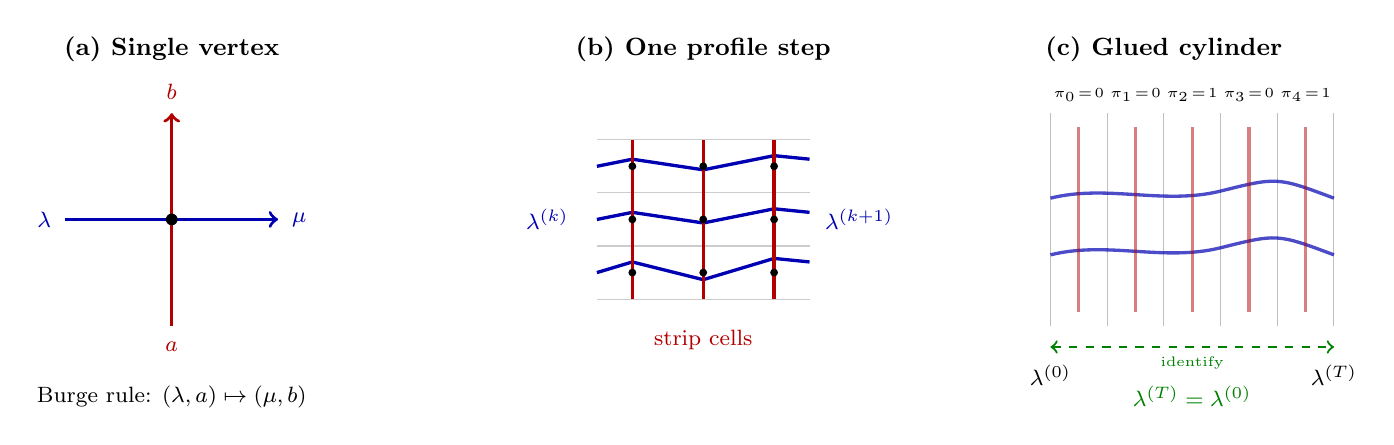
\begin{tikzpicture}[scale=0.9,
  hpath/.style={very thick, blue!70!black},
  vpath/.style={very thick, red!70!black},
  vertex/.style={fill=black, circle, inner sep=1.5pt},
  label/.style={font=\footnotesize}]

%% --- (a) Single vertex ---
\begin{scope}[shift={(-5.5,0)}]
\node[font=\small\bfseries] at (0,2.4) {(a) Single vertex};

% Horizontal path (blue)
\draw[hpath, ->] (-1.5,0) -- (1.5,0);
\node[label, blue!70!black] at (-1.8,0) {$\lambda$};
\node[label, blue!70!black] at (1.8,0) {$\mu$};

% Vertical path (red)
\draw[vpath, ->] (0,-1.5) -- (0,1.5);
\node[label, red!70!black] at (0,-1.8) {$a$};
\node[label, red!70!black] at (0,1.8) {$b$};

% Vertex
\node[vertex] at (0,0) {};

% Label
\node[label] at (0,-2.5) {Burge rule: $(\lambda,a) \mapsto (\mu,b)$};
\end{scope}

%% --- (b) One profile step (strip) ---
\begin{scope}[shift={(2,0)}]
\node[font=\small\bfseries] at (0,2.4) {(b) One profile step};

% Grid
\foreach \i in {0,1,2,3} {
  \draw[gray!40] (-1.5,\i*0.75 - 1.125) -- (1.5,\i*0.75 - 1.125);
}
\foreach \j in {-1,0,1} {
  \draw[gray!40] (\j*1.0, -1.125) -- (\j*1.0, 1.125);
}

% Horizontal paths (blue) — partition boundaries evolving
\draw[hpath] (-1.5,-0.75) -- (-1,{-0.75+0.15})
  -- (0,{-0.75-0.1}) -- (1,{-0.75+0.2}) -- (1.5,-0.6);
\draw[hpath] (-1.5,0) -- (-1,0.1)
  -- (0,-0.05) -- (1,0.15) -- (1.5,0.1);
\draw[hpath] (-1.5,0.75) -- (-1,0.85)
  -- (0,0.7) -- (1,0.9) -- (1.5,0.85);

% Vertical paths (red) — strip data
\draw[vpath] (-1,-1.125) -- (-1,1.125);
\draw[vpath] (0,-1.125) -- (0,1.125);
\draw[vpath] (1,-1.125) -- (1,1.125);

% Vertices at crossings
\foreach \j in {-1,0,1} {
  \foreach \yy in {-0.75,0,0.75} {
    \node[vertex, inner sep=1pt] at (\j,\yy) {};
  }
}

% Labels
\node[label, blue!70!black] at (-2.2,0) {$\lambda^{(k)}$};
\node[label, blue!70!black] at (2.2,0) {$\lambda^{(k+1)}$};
\node[label, red!70!black] at (0,-1.7) {strip cells};

\end{scope}

%% --- (c) Cylindric gluing ---
\begin{scope}[shift={(8.5,0)}]
\node[font=\small\bfseries] at (0,2.4) {(c) Glued cylinder};

% Draw T=5 strips
\foreach \k in {0,1,2,3,4} {
  \pgfmathsetmacro{\x}{\k*0.8 - 1.6}
  \draw[gray!50] (\x,-1.5) -- (\x,1.5);
}
\draw[gray!50] (2.4,-1.5) -- (2.4,1.5);

% Profile labels
\foreach \k/\lab in {0/0, 1/0, 2/1, 3/0, 4/1} {
  \pgfmathsetmacro{\x}{\k*0.8 - 1.2}
  \node[font=\tiny] at (\x,1.75) {$\pi_{\k}\!=\!\lab$};
}

% Horizontal paths wrapping around (blue)
\draw[hpath, opacity=0.7]
  (-1.6,-0.5) .. controls (-0.8,-0.3) and (0,-0.6) ..
  (0.8,-0.4) .. controls (1.6,-0.2) .. (2.4,-0.5);
\draw[hpath, opacity=0.7]
  (-1.6,0.3) .. controls (-0.8,0.5) and (0,0.2) ..
  (0.8,0.4) .. controls (1.6,0.6) .. (2.4,0.3);

% Vertical paths at each step (red)
\foreach \k in {0,1,2,3,4} {
  \pgfmathsetmacro{\x}{\k*0.8 - 1.2}
  \draw[vpath, opacity=0.5] (\x,-1.3) -- (\x,1.3);
}

% Periodic identification arrows
\draw[thick, <->, dashed, green!50!black]
  (-1.6,-1.8) -- node[below, font=\tiny] {identify} (2.4,-1.8);

% Labels
\node[label] at (-1.6,-2.2) {$\lambda^{(0)}$};
\node[label] at (2.4,-2.2) {$\lambda^{(T)}$};
\node[label, green!50!black, font=\footnotesize] at (0.4,-2.5)
  {$\lambda^{(T)} = \lambda^{(0)}$};

\end{scope}

\end{tikzpicture}
\end{center}
\caption{The crossing-path model.
  \textbf{(a)}~A single vertex: a horizontal path (blue,
  partition boundary) crosses a vertical path (red, strip cell).
  The Burge local rule determines the outgoing states $(\mu, b)$
  from the incoming states $(\lambda, a)$.
  \textbf{(b)}~One profile step: multiple horizontal paths
  (evolving partition boundaries) cross multiple vertical paths
  (cells of the horizontal strip).
  \textbf{(c)}~The glued cylinder ($T = 5$ steps, profile
  $\pi = 00101$): both families run all the way around; the left
  and right boundaries are identified.  The intermediate partitions
  $\lambda^{(1)}, \ldots, \lambda^{(T-1)}$ are not part of the
  input---they emerge from the path configuration.}
\label{fig:crossing-paths}
\end{figure}

\begin{definition}[Crossing-path configuration]
\label{def:crossing-config}
A \emph{crossing-path configuration} on the cylinder with
profile~$\pi$ consists of:
\begin{enumerate}
\item a family of horizontal paths wrapping around the cylinder
  (encoding the evolving partition boundaries), and
\item a family of vertical paths threading through the growth
  diagram (encoding the strip data at each profile step),
\end{enumerate}
subject to the Burge crossing rule at every intersection point,
and the \textbf{periodic boundary condition}: the horizontal paths
close up after $T$ steps (i.e.\ $\lambda^{(T)} = \lambda^{(0)}$).
\end{definition}

\begin{proposition}\label{prop:crossing-schur}
The Schur coefficient of $\GK_c$ is a \emph{single count}:
\[
  \langle s_\kappa, \GK_c \rangle
  = \#\bigl\{\text{crossing-path configurations on the cylinder
    with output shape } \kappa \bigr\},
\]
where the ``output shape'' is read from the vertical paths
(the total shape of the cells added across all profile steps).
\end{proposition}

This eliminates the intermediate partitions from the
description: they are determined by the paths at the strip
boundaries, and summing over all cyclic chains is equivalent to
summing over all valid path configurations in the interior.

Note that individual cylindric Schur functions $s_{\lambda/d/\mu}$
are \textbf{not} always Schur-positive
(McNamara~\cite{mcnamara-2006}), but the full
$\GK_c = \sum s_{\lambda/d/\mu}$ is, because the crossing-path
count is manifestly nonneg.

\begin{remark}[Vertex model interpretation]
\label{rem:vertex-model-paths}
The crossing-path model is a \emph{vertex model} on the cylinder.
Each crossing of a horizontal path with a vertical path is a
\emph{vertex} with a local state determined by the incoming path
segments.  The Burge rule assigns admissibility (Boltzmann
weight~$1$ or~$0$) to each vertex.  The periodic boundary condition
makes $\GK_c$ a \emph{transfer matrix trace}, and the Schur
coefficient $\langle s_\kappa, \GK_c \rangle$ is the
partition function restricted to configurations with winding
data~$\kappa$.

This connects to Korff's integrable model for cylindric
partitions~\cite{korff-2011}, where GK is realised as a partition
function of the $\widehat{\mathfrak{sl}}_r$ vertex model, and to
the R-matrix framework of Section~\ref{sec:vertex-model}.
\end{remark}

\subsection{Local rules, R-matrices, and Littlewood--Richardson coefficients}
\label{sec:local-rules-R-matrix}

% 2026-02-18: New subsection — the Zinn-Justin dictionary between
% growth-diagram local rules and integrable vertex models, with
% application to LR coefficients.  Based on arXiv:0809.2392, Section 5.

The crossing-path model (Definition~\ref{def:crossing-config})
is our growth-diagram language for the same object that
Zinn-Justin~\cite{zinn-justin-2009} studies from the
integrable-systems side.  This subsection makes the dictionary
explicit: the local rule \emph{is} an R-matrix, commutativity
of local rules \emph{is} the Yang--Baxter equation, and the
LR coefficient $c^\lambda_{\mu\nu}$ \emph{is} the partition
function of a vertex model on a triangle.

\subsubsection*{The tiling model on the triangular lattice}

Zinn-Justin works on a triangular lattice with two species of
colored paths:
\begin{itemize}
\item \textbf{Green paths} (our ``horizontal'' family):
  move one half-step to the right at each time step.
  In our language, these are the evolving partition boundaries.
\item \textbf{Red paths} (our ``vertical'' family):
  move one half-step to the left at each time step.
  In our language, these encode the strip data (which cells
  are added/removed at each profile step).
\end{itemize}
Each edge of the lattice carries a state from
$\{-, +, 0\}$ (empty, green, red), and each vertex is a
\emph{tile} whose admissibility and weight are determined by
the four surrounding edge states.

The key tiles:
\begin{center}
\renewcommand{\arraystretch}{1.3}
\begin{tabular}{l|l|c}
  \textbf{Tile type} & \textbf{Description} & \textbf{Weight} \\
  \hline
  $\alpha_\pm$ & Same-color lines propagate straight through & $1$ \\
  $\beta_\pm$ & Opposite-color lines cross & $1$ \\
  $\gamma_\pm$ & A line moves in the ``wrong'' direction
    (interaction) & $u$ \\
  $\gamma_0$ & Green and red pass through each other
    transparently & $1$
\end{tabular}
\end{center}
In the unweighted (Schur) case, $u = 0$: the interaction tiles
$\gamma_\pm$ are forbidden, and the model reduces to free
propagation with crossings---precisely the admissibility
condition of our Burge local rule.

\subsubsection*{The R-matrix}

The Boltzmann weights at each vertex assemble into an
\textbf{R-matrix} $R(x)$: a linear map
$R(x) : V \otimes V \to V \otimes V$ where $V = \mathbb{C}^3$
(the three edge states $\{-, +, 0\}$).
The matrix is mostly $\{0, 1\}$-valued; the only entry depending
on the spectral parameter~$x$ is
\[
  R_{(-,+)}^{(-,+)}(x) = x,
\]
corresponding to the interaction tile $\gamma$.
Setting $x = 0$ recovers the \textbf{bijective} local rule:
each legal input $(\alpha, \beta)$ has exactly one legal output
$(\lambda, m)$ with nonzero weight.

\subsubsection*{The Yang--Baxter equation is commutativity of local rules}

The R-matrix satisfies the \textbf{Yang--Baxter equation}
(star-triangle relation): for spectral parameters satisfying
$x + y + z = 0$,
\[
  R_{12}(x)\, R_{13}(y)\, R_{23}(z)
  = R_{23}(z)\, R_{13}(y)\, R_{12}(x).
\]
This is the integrable-systems version of the commutativity
property
$\mathfrak{L}_i \circ \mathfrak{L}_j
= \mathfrak{L}_j \circ \mathfrak{L}_i$ for $|i-j| \geq 2$
(Section~\ref{sec:local-rules}).

In the growth-diagram proof of Borodin's identity
(Section~\ref{sec:growth-diagram}), this commutativity ensures
that the growth diagram is \emph{well-defined} regardless of
the order in which rows are processed.
In Zinn-Justin's language, the same property ensures that
the \emph{transfer matrices commute}:
\[
  [\widetilde{T}_+(u),\, \widetilde{T}_-(v)] = 0,
  \qquad
  [\widetilde{T}_\pm(u),\, T] = 0,
  \qquad
  [\widetilde{T}_+(u),\, \widetilde{T}_+(v)] = 0.
\]
The proof is the standard ``RTT = TTR'' argument: insert an
R-matrix at one end of a product of two transfer matrices, use
the Yang--Baxter equation to push it across row by row, and
remove it at the other end.

\begin{center}
\renewcommand{\arraystretch}{1.4}
\begin{tabular}{l|l}
  \textbf{Our growth diagram}
    & \textbf{Zinn-Justin's vertex model} \\
  \hline
  Vertex of the grid
    & Vertex of the triangular lattice \\
  Input partitions $(\alpha, \beta)$
    & Input edge states \\
  Output $(\lambda, m)$
    & Output edge states \\
  Burge rule $\mathfrak{U}_{\alpha,\beta}(m,\mu) = \lambda$
    & R-matrix entry $R^{(\lambda,m)}_{(\alpha,\beta,\mu)}$ \\
  Weight $|\lambda| = m + |\alpha| + |\beta| - |\mu|$
    & Boltzmann weight \\
  Commutativity ($|i - j| \geq 2$)
    & Yang--Baxter equation \\
  Growth diagram = bijection CPP $\leftrightarrow$ ALCD
    & Transfer matrix trace = partition function \\
  Schur, all weights $\in \{0,1\}$
    & $x = 0$: free fermion limit
\end{tabular}
\end{center}

\subsubsection*{LR coefficients as a partition function on a triangle}

The payoff of Zinn-Justin's framework is a direct, algebraic
proof that $c^\lambda_{\mu\nu}$ counts puzzle tilings.
The argument (Section~5 of~\cite{zinn-justin-2009}) proceeds
in five steps:

\begin{enumerate}
\item \textbf{Start from the supersymmetric Schur function.}
  Express $s_\lambda(u_1, \ldots, u_m / v_1, \ldots, v_n)$
  as a transfer-matrix expectation value:
  \[
    s_\lambda(\mathbf{u}/\mathbf{v})
    = \langle \varnothing \,|\,
    \textstyle\prod_i \widetilde{T}_+(u_i)\,
    \prod_j \widetilde{T}_-(v_j)
    \,|\, \lambda \rangle.
  \]

\item \textbf{Evolve the state $|\lambda\rangle$ forward.}
  Apply the (parameter-free) transfer matrix $T$ repeatedly.
  After $2k$ steps (for $k$ large enough), the state
  decomposes into spatially separated components:
  \[
    T^{2k} |\lambda\rangle
    = \sum_{\mu,\nu} c^\lambda_{\mu\nu}\;
    |\mu\rangle \sqcup_k |\nu\rangle,
  \]
  where $|\mu\rangle \sqcup_k |\nu\rangle$ means the green
  particles encoding~$\mu$ have moved far to the left and the
  red particles encoding~$\nu$ have moved far to the right.
  The coefficients $c^\lambda_{\mu\nu}$ are defined by this
  expansion.

\item \textbf{Use commutativity to separate.}
  Since all transfer matrices commute (Yang--Baxter!), move
  $T^{2k}$ past the $\widetilde{T}_\pm$ operators:
  \[
    s_\lambda(\mathbf{u}/\mathbf{v})
    = \sum_{\mu,\nu} c^\lambda_{\mu\nu}\;
    \langle \varnothing \,|\,
    \textstyle\prod_i \widetilde{T}_+(u_i)\,
    \prod_j \widetilde{T}_-(v_j)
    \,|\, \mu \rangle \sqcup_k |\nu\rangle.
  \]

\item \textbf{Factor into independent Schur functions.}
  Since $|\mu\rangle$ and $|\nu\rangle$ are spatially
  separated, the expectation value factors:
  \[
    s_\lambda(\mathbf{u}/\mathbf{v})
    = \sum_{\mu,\nu} c^\lambda_{\mu\nu}\;
    s_\nu(u_1, \ldots, u_m)\;
    s_{\mu^{\mathrm{T}}}(v_1, \ldots, v_n).
  \]

\item \textbf{Identify the coefficients.}
  The LHS is the supersymmetric Schur function, whose expansion
  in products of ordinary Schur functions is unique.
  Therefore $c^\lambda_{\mu\nu}$ \emph{are} the
  Littlewood--Richardson coefficients.
\end{enumerate}

\begin{remark}[The triangle]\label{rem:triangle}
The evolution $T^{2k}|\lambda\rangle$ takes place entirely
within a finite triangular region of the lattice: green particles
drift left, red particles drift right, and after enough steps they
separate.  The Young diagrams $\mu$ and $\nu$ are read from the
binary sequences of particles on the two upper edges of the
triangle.  Therefore $c^\lambda_{\mu\nu}$ counts the number of
valid \textbf{tilings of the triangle} with boundary data
$(\lambda, \mu, \nu)$---these are precisely the
\emph{puzzles} of Knutson--Tao~\cite{knutson-tao-2003}.
\end{remark}

\begin{remark}[Why this matters for us]\label{rem:why-this-matters}
The crossing-path model on the cylinder
(Proposition~\ref{prop:crossing-schur}) writes
$\langle s_\kappa, \GK_c \rangle$ as a count of path
configurations.  Each ``strip'' of the cylinder contributes an
LR coefficient, which by the above is a puzzle count.
The full cylindric generating function is thus a
\textbf{transfer matrix trace} over puzzle partition functions.

This is the starting point for the $(q,t)$-deformation
programme (Section~\ref{sec:vertex-model}): replace the
$\{0,1\}$-valued Boltzmann weights with polynomial
$(q,t)$-weights, turning counting into a weighted generating
function.  The Yang--Baxter equation guarantees that the
resulting $(q,t)$-LR coefficients are well-defined
(independent of the lattice decomposition), and if the
Boltzmann weights are nonneg polynomials, positivity follows
for free.
\end{remark}


%% ================================================================
\part{Open Problems}
\label{part:problems}
%% ================================================================

%% ==================================================================
\section{Warnaar's Conjecture and the ground-set formulation}
\label{sec:conjecture}
%% ==================================================================

\subsection{The $Q$-polynomial}

\begin{definition}\label{def:Q}
The \emph{$Q$-polynomial} is
\begin{equation}\label{eq:Q-def}
  Q_{n,c}(q)
  = \qpochn{q}{q}{n}
    \cdot [z^n]\bigl(\qpoch{zq}{q} \cdot \GK_c(z,q)\bigr).
\end{equation}
\end{definition}

\begin{conjecture}[Warnaar~\cite{warnaar-2021}, Conjecture~2.7]
\label{conj:main}
For all $n \geq 0$ and all rank-3 profiles $c$ with
$d \not\equiv 0 \pmod{3}$, one has
$Q_{n,c}(q) \in \N[q]$.
\end{conjecture}

% 2026-02-16: Clarified rank-3 restriction and added A_r conjecture
\begin{remark}[Why rank~3?]\label{rem:why-rank3}
Conjecture~\ref{conj:main} is the $A_2$ case ($r = 3$) of a
general conjecture for all ranks.
The Andrews--Gordon identities for $A_1$ ($r = 2$) are classical,
and the $Q$-polynomials reduce to $q^{n^2}$ or $q^{n(n+1)}$
(see Section~\ref{sec:dead-ends}).
The $A_2$ case is the first genuinely open case.
\end{remark}

\begin{conjecture}[Warnaar~\cite{warnaar-2021}, Conjecture~8.4:
general rank]
\label{conj:general-rank}
Fix $d, r \geq 1$ and a profile $c = (c_0, \ldots, c_{r-1})$
of level~$d$ (i.e.\ $c_0 + \cdots + c_{r-1} = d$).
Then $Q_{n,c}(q) \in \N[q]$ and
\begin{equation}\label{eq:Q-at-1-general}
  Q_{n,c}(1)
  = \left(
    \frac{\gcd(d,r)}{d+r}\binom{d+r}{r} - \gcd(d,r)
  \right)^{\!n}.
\end{equation}
\end{conjecture}

\begin{remark}[Recovering the $A_2$ case]
For $r = 3$ and $\gcd(d,3) = 1$, formula~\eqref{eq:Q-at-1-general}
gives
$Q_{n,c}(1) = \bigl(\tfrac{1}{d+3}\binom{d+3}{3} - 1\bigr)^n
= \bigl(\tfrac{(d+1)(d+2)}{6} - 1\bigr)^n$,
matching Conjecture~\ref{conj:main}.
For $r = 4$, $d = 7$: $Q_{n,c}(1) = (\tfrac{1}{11}\binom{11}{4} - 1)^n
= 29^n$.
The polynomiality and the $q = 1$ evaluation have been
established by Welsh~\cite{welsh-2021}; the
\textbf{nonnegativity of coefficients} remains open.
\end{remark}

\begin{remark}[The $d \equiv 0 \pmod{3}$ exclusion]\label{rem:d-mod3}
Warnaar excludes $d \equiv 0 \pmod{3}$ from the conjecture.
Computationally, the cyclic descent injection
(Section~\ref{sec:cyclic-descent}) fails for $d \equiv 0 \pmod{3}$
because the balanced slack $(d/3, d/3, d/3)$ has empty
cyclic descent set.
For $d = 3$, the triple count per weight oscillates
$(3,3,4,3,3,4,\ldots)$, preventing any uniform injection.
However, direct computation (see below) shows that $Q_{n,c}(q)$
is \emph{still nonneg} for $d \equiv 0 \pmod{3}$; the issue is
that $Q_n(1)$ is no longer a fixed power $K^n$ independent
of the profile.
\end{remark}

% 2026-02-16: Computation result for d ≡ 0 mod 3
\begin{observation}\label{obs:d0mod3}
For all six profiles tested with $d = 3$ and $d = 6$
($n \leq 3$, $\max\_w = 20$),
$Q_{n,c}(q)$ has nonneg integer coefficients.
Representative data ($d = 3$, $c = (1,1,1)$):
\begin{center}
\begin{tabular}{c|l|c}
$n$ & $Q_{n,c}(q)$ & $Q_n(1)$ \\\hline
$0$ & $1$ & $1$ \\
$1$ & $2q + 2q^2 + 3q^3$ & $7$ \\
$2$ & $q^3 + 3q^4 + 4q^5 + 7q^6 + \cdots + 3q^{12}$ & $49$ \\
$3$ & $2q^7 + 2q^8 + 6q^9 + \cdots$ & $277$
\end{tabular}
\end{center}
The crucial difference from $d \not\equiv 0 \pmod{3}$:
$Q_3(1) = 277 \neq 7^3 = 343$, and $Q_3(1)$ depends
on the profile ($(2,1,0) \to 218$, $(3,0,0) \to 134$).
\end{observation}

Computationally verified for $d = 1,2,4,5,7$
(10 profiles, all pass).
For $d = 2$: $Q_n$ is a monomial---$q^{n^2}$ (first
Rogers--Ramanujan) or $q^{n(n+1)}$ (second RR identity).

\subsection{Derivation: the $(S, U, \nu)$ ground set}

ALSO DO THE DERIVSTION OF THE $(S,\nu)$ GROUND SET
EXPANDING IN TERMS OF THE $h_m$.

WHAT IS THE QUASI-SYMMETRIC ANALOG OF THE $h_m$

Expanding the three factors in~\eqref{eq:Q-def}---Euler's
identity for $\qpoch{zq}{q}$, the $q$-binomial interpretation
of $\qpochn{q}{q}{n}/\qpochn{q}{q}{j}$, and the subset expansion
of $\qpochn{q}{q}{m}$---yields:

\begin{proposition}\label{prop:ground-set}
\begin{equation}\label{eq:ground-set}
  Q_{n,c}(q) = \sum_{j=0}^{n}\;
  \sum_{\substack{S \subseteq \{1,\ldots,n\} \\ |S|=j}}\;
  \sum_{U \subseteq \{1,\ldots,n-j\}}\;
  \sum_{\substack{\nu \in \CPP(c) \\ \max(\nu) = n-j}}
  (-1)^{|S|+|U|}\, q^{\sigma(S)+\sigma(U)+|\nu|},
\end{equation}
where $\sigma(S) = \sum_{s \in S} s$.
\end{proposition}

\begin{proof}[Proof sketch]
Use $q^{j(j+1)/2}\qbin{n}{j} = \sum_{|S|=j} q^{\sigma(S)}$
and $\qpochn{q}{q}{m} = \sum_{U \subseteq [m]} (-1)^{|U|}
q^{\sigma(U)}$, then combine with $g_m = \sum_{\max(\nu)=m} q^{|\nu|}$.
\end{proof}

The sign is $(-1)^{|S|+|U|}$; the conjecture asserts that the
total signed weight at each $q$-power is nonneg.
The three components play distinct roles:
\begin{itemize}
  \item $S \subseteq \{1,\ldots,n\}$ with $|S| = j$: selects
    which ``paths'' (level sets) to remove;
    the $q$-binomial $q^{j(j+1)/2}\qbin{n}{j}$ counts these
    subsets by $\sigma(S)$.
  \item $U \subseteq \{1,\ldots,n-j\}$: the $(q)_{n-j}$ factor
    creates an alternating sum over subsets of remaining paths.
  \item $\nu \in \CPP(c)$ with $\max(\nu) = n-j$: the cylindric
    partition with $n-j$ paths.
\end{itemize}

\subsection{The $q$-binomial decomposition}

Define $h_m = \qpochn{q}{q}{m} \cdot g_m$
(the ``corrected'' coefficients). Then:
\begin{equation}\label{eq:q-binom-forward}
  Q_n = \sum_{j=0}^{n} (-1)^j\, q^{\binom{j+1}{2}}\,
    \qbin{n}{j}\, h_{n-j},
\end{equation}
with inverse
\begin{equation}\label{eq:q-binom-inverse}
  h_m = \sum_{k=0}^{m} q^k\, \qbin{m}{k}\, Q_{m-k}.
\end{equation}
The $h_m$ are nonneg polynomials for all tested profiles
($d = 1,2,4,5,7$).
By~\eqref{eq:q-binom-inverse}, $Q_n \geq 0$ implies $h_m \geq 0$
(all terms are nonneg); the converse fails because
\eqref{eq:q-binom-forward} is an alternating sum.

% 2026-02-16: h_m positivity is combinatorially transparent
\begin{remark}[$h_m$ positivity is combinatorially clear]\label{rem:hm-trivial}
  The positivity of~$h_m$ should \textbf{not} be regarded as deep.
  From the NILP / growth-diagram perspective, $h_m$~counts a
  subset of \emph{arbitrarily labelled} cylindric diagrams:
  a CPP with max entry~$m$ is a cylindric diagram (the support)
  together with a labelling of its cells by values in
  $\{1,\ldots,m\}$ subject to interlacing conditions.
  Multiplying $g_m$ by~$\qpochn{q}{q}{m}$ restricts to
  a finite sub-collection of such labellings (analogous to
  the passage from semistandard to standard fillings in the
  P-partition framework, where $(q)_p \cdot \Omega_P(q) = W_P(q)$
  counts strict $P$-partitions).
  The result is manifestly a generating function with nonneg
  coefficients.

  This perspective comes from the growth-diagram / Burge
  local-rule toolkit and may not be apparent from the
  $q$-series viewpoint, where multiplying by the alternating
  polynomial~$\qpochn{q}{q}{m}$ has no obvious reason to
  preserve positivity.

  \textbf{The hard problem} is the alternating $q$-binomial
  sum~\eqref{eq:q-binom-forward}: even with $h_m \geq 0$
  as input, the signs $(-1)^j$ produce massive cancellation
  that must resolve to a nonneg polynomial~$Q_n$.
  Proving Conjecture~\ref{conj:main} requires explaining
  \emph{this} cancellation, not the positivity of~$h_m$.
\end{remark}

% 2026-02-16: Added crush and drop definitions
\begin{definition}[Drop and crush]\label{def:crush-drop}
Let $\mathfrak{c}$ be a CPP with max entry~$n$
(equivalently, $n$ non-intersecting lattice paths).
\begin{itemize}
\item \textbf{Drop level~$k$} ($1 \leq k \leq n$):
  remove the $k$-th path (counting from the bottom).
  In the labelled diagram, replace every label $r \geq k$
  with $r - 1$.
  The result has max entry $\leq n-1$.
  On the frequency GF, drop acts as
  $z_r \mapsto z_{r-1}$ for all $r \geq k$.
\item \textbf{Crush level~$k$} ($1 \leq k \leq n$):
  push the $k$-th path flush against the $(k+1)$-th path above it.
  In the labelled diagram, replace every label equal to~$k$ with $k-1$.
  The result has max entry $\leq n$ but the $k$-th and
  $(k-1)$-th paths may merge.
  Crush decreases the weight by $\#_k(\mathfrak{c})$
  (the number of cells with value~$k$), which \textbf{varies}
  across CPPs.
\end{itemize}
\end{definition}

\begin{remark}[NILP interpretation of $(S,U)$]
Starting with a CPP with max entry~$n$, the set~$S$ (with $|S|=j$)
selects $j$ paths to \emph{drop}.  This leaves a CPP with max entry
$n-j$.  The set~$U \subseteq \{1,\ldots,n-j\}$ then selects
paths to \emph{crush}.  The result is a CPP~$\nu$ with
$\max(\nu) = n - j$.  However, crush does \textbf{not preserve
weight} (each crush removes a variable number of boxes),
so this map is not invertible and does not yield a sign-reversing
involution.
\end{remark}

I WILL DRAW THE DIAGRAMS FOR THIS, IT REALLY BELONGS IN THE
DEAD END SECTION

\subsection{Multivariate $q$-analog: non-positivity}
\label{sec:multivariate-failure}

% 2026-02-17: Rewritten per author instructions — multivariate formulation
A natural refinement replaces the univariate weight $q^{|\nu|}$
of a CPP with per-value variables: if $\nu$ has $f_k$ cells of
value~$k$, set $q_\nu = q_1^{f_1}\, q_2^{f_2}\, \cdots\,$.
The specialisation $q_k \mapsto q^k$ recovers $q^{|\nu|}$.
Defining $Q_{n,c}(q_1, q_2, \ldots)$ via the corresponding
multivariate substitution in~\eqref{eq:Q-def}, the coefficients
of the monomials~$q_\mu$ are \textbf{not nonneg} for $n \geq 2$.
The positivity of $Q_{n,c}(q)$ does \emph{not} lift to this
multivariate refinement.
(See \texttt{scripts/qsym\_Q\_polynomial.py}.)

\begin{remark}
This per-value refinement is \emph{not} the same as
Borodin's multivariable extension of the product formula,
which tracks diagonal weights (one variable per diagonal of the
cylindric diagram) rather than per-value frequencies.
\end{remark}

% 2026-02-16: Two-level reformulation
\subsection{Sharpened formulation: the $(S, \nu')$ involution problem}
\label{sec:two-level}

Since $h_m \geq 0$ is combinatorially clear
(Remark~\ref{rem:hm-trivial}), the three-level $(S,U,\nu)$
ground set~\eqref{eq:ground-set} can be collapsed to a
\textbf{two-level} problem.
The $U$-factor is absorbed:
\[
  \sum_{U \subseteq [n-j]} (-1)^{|U|}\, q^{\sigma(U)}
  \cdot \sum_{\max(\nu) = n-j} q^{|\nu|}
  \;=\; \qpochn{q}{q}{n-j} \cdot g_{n-j}
  \;=\; h_{n-j} \;\geq\; 0.
\]
Write $h_m = \sum_{\nu'} q^{|\nu'|}$, where $\nu'$~ranges over
the \emph{restricted labelled cylindric diagrams} counted by~$h_m$.
Then equation~\eqref{eq:q-binom-forward} becomes
\begin{equation}\label{eq:two-level}
  Q_n = \sum_{j=0}^{n}\;
  \sum_{\substack{S \subseteq [n] \\ |S| = j}}\;
  \sum_{\nu'}
  (-1)^j\, q^{\sigma(S) + |\nu'|},
\end{equation}
where $\nu'$ ranges over restricted labellings with
max entry~$n - j$.
The conjecture is equivalent to the existence of a
\textbf{sign-reversing involution}
$(S, \nu') \mapsto (S', \nu'')$
with:
\begin{enumerate}
  \item $|S'| = |S| \pm 1$ (to flip $(-1)^j$),
  \item $\sigma(S') + |\nu''| = \sigma(S) + |\nu'|$
    (weight-preserving),
  \item fixed points all have even $|S|$
    (so the residual sum is nonneg).
\end{enumerate}

\begin{remark}[Why this is cleaner]
The three-level approach failed because the $U$-toggle involution
produced cross-cancellation between different QSym monomials
(\S\ref{sec:multivariate-failure}).  By absorbing the $U$-level
into the combinatorially-transparent $h_m$, we avoid that issue
entirely.  The involution now operates only on~$S$ (which paths
to drop), adjusting $\nu'$ (the restricted labelling) to
compensate the weight change.  In the NILP picture:
adding or removing one path from~$S$ changes $\sigma(S)$
by the index of the path and changes $\nu'$ from a labelling
with max entry~$n-j$ to one with max entry~$n-j \mp 1$.
\end{remark}


%% ==================================================================
\section{The disconnect --- why $L$-positivity does not imply $Q$-positivity}
\label{sec:disconnect}
%% ==================================================================


Despite these strong properties, the $\QSym$ structure does
\emph{not} help with Conjecture~\ref{conj:main}:
\begin{enumerate}
  \item The max-entry statistic $n(\pi) = \max\{k : \#_k > 0\}$
    is not a monomial specialisation of the $z_k$;
  \item The E--H factorisation does not lift to $\QSym$: both
    $\prod(1 - tz_k) \cdot \widetilde{\GK}_c$ (with max-entry
    variable) and $\prod(1 - z_k) \cdot \widetilde{\GK}_c$
    (without) have negative coefficients;
  \item Cross-cancellation between different frequency vectors
    (\S\ref{sec:multivariate-failure}) is essential.
\end{enumerate}

The positivity of $Q_{n,c}(q)$ is an \emph{intrinsically
one-variable} phenomenon.


%% ==================================================================
\section{Partial quasi-symmetry and the max-entry refinement}
\label{sec:partial}
%% ==================================================================

\subsection{CPPs with max $= n$ as $\Z[z_1,\ldots,z_{n-1}][z_n]$}

Write $\tilde{g}_n = \sum_{\max(\pi)=n} z_1^{\#_1} \cdots z_n^{\#_n}$
for CPPs with exact max entry~$n$. This is \emph{not}
quasi-symmetric in $z_1, \ldots, z_n$ (the value $n$ is privileged).
However:

\begin{observation}[Verified: 55 profiles, $n \leq 3$]
\label{obs:partial}
Writing $\tilde{g}_n = \sum_{m \geq 1} z_n^m \cdot
f_{n,m}(z_1, \ldots, z_{n-1})$, each slice $f_{n,m}$ is
quasi-symmetric in $z_1, \ldots, z_{n-1}$:
\[
  \tilde{g}_n \in z_n \cdot \QSym(z_1, \ldots, z_{n-1})[z_n].
\]
\end{observation}

Slice $M$-positivity holds (coefficients count CPPs), but
\textbf{slice $L$-positivity fails} at $n \geq 3$: the
$M$-coefficients satisfy $a_{(k)} > a_{(j,k)}$, forcing
$L_{(a,b)} = M_{(a,b)} - M_{(a+b)} < 0$.

\subsection{Variable-count mismatch}

The E--H factorisation couples objects in incompatible
numbers of variables: $\qpochn{q}{q}{n}$ lifts to
$\prod_{k \geq 1}(1 - z_k)$ (infinitely many variables),
while $\tilde{g}_n$ is a polynomial in only $z_1, \ldots, z_n$.
This structural mismatch obstructs any multivariate lift of
$Q_{n,c}$.

\subsection{RPPs with max~$n$ and RSK}

% 2026-02-16: Added proof sketch for RPP formula
For reverse plane partitions (RPPs) of shape~$\lambda$:
\begin{equation}\label{eq:rpp-schur}
  \sum_{\substack{\pi \in \RPP(\lambda) \\ \max(\pi) \leq n}}
  q^{|\pi|}
  = s_\lambda(1, q, \ldots, q^{n-1}).
\end{equation}

\begin{proof}[Proof sketch]
An RPP of shape~$\lambda$ with max entry $\leq n$ is the
same as a semistandard Young tableau (SSYT) of shape~$\lambda$
with entries in $\{0, 1, \ldots, n-1\}$ (with weakly increasing
rows and columns, read as an RPP).
By the combinatorial definition of the Schur function,
$s_\lambda(x_1, \ldots, x_n) = \sum_{T \in \SSYT(\lambda, n)} x^T$.
Setting $x_k = q^{k-1}$ for $k = 1, \ldots, n$ gives weight
$q^{|\pi|}$ to each RPP~$\pi$, yielding~\eqref{eq:rpp-schur}.
\end{proof}

The exact max-$n$ count is thus
$g_{n,\lambda} = s_\lambda(1, q, \ldots, q^{n-1})
- s_\lambda(1, q, \ldots, q^{n-2})$,
manifestly nonneg since it counts objects (RPPs with max
entry \emph{exactly}~$n$).
Under RSK, max entry $= n$ means $n$ rows in the growth diagram,
$\max(P) = n$ in the insertion tableau, and an alphabet of
size~$n$ for the Schur function.

For CPPs the analogous extraction is \emph{not} a simple difference
but involves the infinite product $(zq;q)_\infty$---this is
precisely where positivity becomes hard.


%% ==================================================================
\section{Connecting $P$-partitions to CPPs}
\label{sec:P-part-cpp}
%% ==================================================================


The CPP interlacing conditions~\eqref{eq:interlacing} are
precisely of $P$-partition type (weak and strict order comparisons
on entries), \emph{except} for the cyclic closure
$\mu^T = \mu^0$.

For any \textbf{fixed max entry} $\leq n$, the poset is acyclic:
the cycle can be ``unrolled'' since all values lie in
$\{0, 1, \ldots, n\}$, and classical $P$-partition theory
applies.  The $L$-coefficients then count linear
extensions of the poset by descent set.

This explains the quasi-symmetry and $L$-positivity of
$\widetilde{\GK}_c$ \emph{degree by degree} (i.e.\ for each
fixed~$n$).  The full $\widetilde{\GK}_c$ is an \emph{infinite
sum} of these contributions, and the fact that an infinite sum
of $L$-positive functions remains $L$-positive is nontrivial
(it holds here because the posets are nested: the max-$n$ poset
is a subposet of the max-$(n+1)$ poset).

However, the cyclic structure is essential for the cylindric
identities, and ``cutting the cycle'' destroys the algebraic
connection to Rogers--Ramanujan-type identities.

\begin{remark}[Why the reading word matters for CPPs]
\label{rem:reading-word-cpp}
Theorem~\ref{thm:P-part-qsym-full} says that $L$-positivity
comes from counting linear extensions by descent set.
A \emph{linear extension} is a \emph{reading word}: a way to
linearly order the elements of the poset.  For ordinary
tableaux, the standard reading word (right to left, top to
bottom) is the natural choice.  For CPPs, the analogous question
is: \textbf{what is the right way to linearly order the cells of
a cylindric plane partition?}  The cyclic structure (the profile
wraps around $\Z/3\Z$) means there is no single canonical
starting point, and different choices may give different descent
sets.  This is the content of
Conjecture~\ref{conj:descent}.
\end{remark}


%% ==================================================================
\section{A $(q,t)$-Macdonald statistic on LR configurations}
\label{sec:vertex-model}
%% ==================================================================


\textbf{Central ambition.}
The Schur coefficients
$\langle s_\kappa, \GK_c \rangle$ are products of
LR coefficients (Section~\ref{sec:trace}).
A long-standing goal is to define a \emph{Macdonald
statistic}---a $(q,t)$-weight on the combinatorial objects
that compute LR coefficients (intersecting lattice paths,
puzzles, hive configurations)---such that:
\begin{itemize}
\item the statistic arises naturally from the
  \emph{plethystic alphabet} $\Omega[(q-t)\,\mathcal{D}]$
  that governs the Macdonald Pieri coefficients
  (Section~\ref{sec:macdonald});
\item the weighted count of LR configurations gives a
  $(q,t)$-analog of the LR coefficient;
\item the cylindric Schur coefficients---being products of
  these $(q,t)$-LR coefficients---inherit positivity.
\end{itemize}

\medskip\noindent\textbf{Why this should work: the pieces already exist.}

\begin{enumerate}
\item \textbf{The plethystic weight is local.}
  Each horizontal strip $\lambda/\mu$ in the interlacing
  sequence carries the Pieri weight
  $\varphi_{\lambda/\mu}(q,t)
  = \Omega[(q-t)(\mathcal{A}_{\lambda/\mu}
  - \mathcal{B}_{\lambda/\mu})]$
  (thesis~\cite{langer-thesis}, Chapter~4).
  In the NILP model, this factorises over \emph{individual
  cubes}: each cube~$s$ contributes
  $\frac{1-q^{a(s)}t^{\ell(s)+1}}{1-q^{a(s)+1}t^{\ell(s)}}$
  depending on whether it is a peak or valley
  (eq.~\eqref{eq:mac-weight}).
  This is a \textbf{local statistic on the lattice path
  configuration}---exactly the kind of data an R-matrix
  encodes.

\item \textbf{Zinn-Justin's integrable tiling framework.}
  Zinn-Justin~\cite{zinn-justin-2009} showed that LR
  coefficients $c_{\lambda\mu}^\nu$ equal the partition
  function of an integrable tiling model: each puzzle piece
  (= vertex of a lattice model) carries a Boltzmann weight,
  and the Yang--Baxter equation ensures the count is
  well-defined. In the \emph{unweighted} (Schur) case,
  all Boltzmann weights are~$1$ or~$0$, and the partition
  function simply \emph{counts} puzzles.

% 2026-02-18: Made the local-rule / R-matrix identification explicit
\item \textbf{The local rule \emph{is} the R-matrix.}
  The Burge local rule
  (Definition~\ref{def:local-rule}, Section~\ref{sec:local-rules})
  and the R-matrix are \textbf{the same mathematical object}
  viewed from two sides:
  \begin{center}
  \renewcommand{\arraystretch}{1.3}
  \begin{tabular}{l|l}
  \textbf{Growth diagram} & \textbf{Lattice model} \\ \hline
  Vertex of the grid & Vertex of the lattice \\
  Input partitions $(\alpha, \beta)$ & Input edge states \\
  Output partition $\lambda$, integer $m$ & Output edge states \\
  Burge local rule $\mathfrak{U}_{\alpha,\beta}(m,\mu)=\lambda$
    & R-matrix entry $R^{(\lambda,m)}_{(\alpha,\beta,\mu)}$ \\
  Weight preservation $|\lambda|=m+|\alpha|+|\beta|-|\mu|$
    & Boltzmann weight \\
  Commutativity $\mathfrak{L}_i \circ \mathfrak{L}_j
    = \mathfrak{L}_j \circ \mathfrak{L}_i$ for $|i-j|\geq 2$
    & Yang--Baxter equation
  \end{tabular}
  \end{center}
  In the crossing-path model (Section~\ref{sec:crossing-paths}),
  this identification is literal: the horizontal path (partition
  boundary) and vertical path (strip cell) cross at a vertex,
  and the Burge rule determines the outgoing states---exactly
  as an R-matrix determines scattering amplitudes.

  \smallskip
  In the Schur (unweighted) case, the local rule is a
  \emph{bijection}: each legal input has exactly one legal output,
  so all Boltzmann weights are~$0$ or~$1$.  The key insight for
  the $(q,t)$-deformation is that replacing the bijective local
  rule with a \emph{weighted} R-matrix---where each vertex
  carries a polynomial Boltzmann weight in $(q,t)$---turns the
  growth diagram from a counting device into a
  \emph{generating function machine}.

  \smallskip
  \textbf{This is already done at the algebraic level.}
  The $(q,t)$-Borodin identity
  (Section~\ref{sec:macdonald}, eq.~\eqref{eq:mac-trace})
  gives a Macdonald analog of Borodin's product formula,
  proved in~\cite{langer-thesis}.
  The Macdonald Pieri coefficients
  $\varphi_{\lambda/\mu}(q,t)$ and
  $\psi_{\lambda/\mu}(q,t)$
  play exactly the role of Boltzmann weights at each vertex of
  the growth diagram: the proof telescopes identically to the
  Schur case, with $1/(1 - u_iu_jw^{m+1})$ replaced by
  $(tu_iu_jw^{m+1};q)_\infty / (u_iu_jw^{m+1};q)_\infty$.
  What remains open is making this identification
  \emph{combinatorially explicit}: expressing $\varphi_{\lambda/\mu}$
  as a product of R-matrix entries over vertices of the crossing-path
  model (Question~\ref{q:pieri-rmatrix}),
  which would upgrade the algebraic identity to a
  vertex-model partition function and open the door to
  positivity via Wheeler's
  framework~\cite{wheeler-zinn-justin-2016,wheeler-zinn-justin-2016b,
  aggarwal-borodin-wheeler-2021}.
  
  % 2026-02-17: Reproduced from arXiv:0809.2392, Figure 8 (triangle.eps)
  % Coordinate map: x=(EPS_x-2100)/600, y=(9300-EPS_y)/600
  \begin{center}
  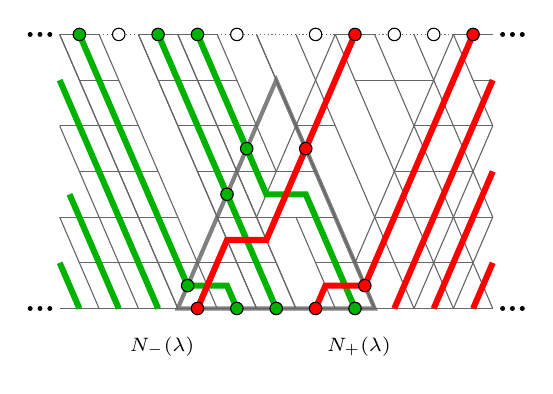
\begin{tikzpicture}[xscale=0.50, yscale=0.58,
    gridline/.style={thin, black!60},
    dashline/.style={thin, black!60, densely dotted},
    triline/.style={line width=1.5pt, black!50},
    gpath/.style={line width=2.2pt, green!70!black},
    rpath/.style={line width=2.2pt, red},
    gdot/.style={circle, fill=green!70!black, draw=black,
                 inner sep=0pt, minimum size=4.5pt},
    rdot/.style={circle, fill=red, draw=black,
                 inner sep=0pt, minimum size=4.5pt},
    wdot/.style={circle, fill=white, draw=black,
                 inner sep=0pt, minimum size=4.5pt},
    edot/.style={circle, fill=black, inner sep=0pt, minimum size=1.8pt}
  ]
    %% ── Triangle boundary ──
    \draw[triline] (3,0) -- (5.5,5) -- (8,0) -- cycle;

    %% ── Horizontal grid lines ──
    \draw[gridline] (0,0) -- (11,0);
    \draw[gridline] (0.5,1) -- (5.5,1);
    \draw[gridline] (6.5,1) -- (10.5,1);
    \draw[gridline] (0,2) -- (3,2);
    \draw[gridline] (4,2) -- (7,2);
    \draw[gridline] (8,2) -- (11,2);
    \draw[gridline] (0.5,3) -- (2.5,3);
    \draw[gridline] (3.5,3) -- (6.5,3);
    \draw[gridline] (8.5,3) -- (10.5,3);
    \draw[gridline] (0,4) -- (2,4);
    \draw[gridline] (3,4) -- (5,4);
    \draw[gridline] (6,4) -- (7,4);
    \draw[gridline] (9,4) -- (11,4);
    \draw[gridline] (0.5,5) -- (1.5,5);
    \draw[gridline] (2.5,5) -- (4.5,5);
    \draw[gridline] (7.5,5) -- (9.5,5);
    \draw[gridline] (10.5,5) -- (11,5);
    %% Top row (y=6): solid + dashed
    \draw[gridline] (0,6) -- (1,6);
    \draw[dashline] (1,6) -- (2,6);
    \draw[gridline] (2,6) -- (4,6);
    \draw[dashline] (4,6) -- (7,6);
    \draw[gridline] (7,6) -- (8,6);
    \draw[dashline] (8,6) -- (10,6);
    \draw[gridline] (10,6) -- (11,6);

    %% ── Diagonal grid lines (from EPS) ──
    %% Left-leaning (NW direction, green particle default)
    \draw[gridline] (3,0) -- (0,6);
    \draw[gridline] (2,0) -- (0,4);
    \draw[gridline] (1,0) -- (0,2);
    \draw[gridline] (5,0) -- (2,6);
    \draw[gridline] (6,0) -- (3,6);
    \draw[gridline] (8,0) -- (5,6);
    \draw[gridline] (4,0) -- (3.5,1);
    \draw[gridline] (7,0) -- (6.5,1);
    \draw[gridline] (5.5,3) -- (4,6);
    \draw[gridline] (5,2) -- (7,6);
    \draw[gridline] (6,2) -- (6.5,1);
    \draw[gridline] (9,0) -- (11,4);
    \draw[gridline] (10,0) -- (11,2);
    \draw[gridline] (10,6) -- (7.5,1);
    %% Right-leaning (NE direction, red particle default)
    \draw[gridline] (0,6) -- (3,0);
    \draw[gridline] (1,6) -- (3.5,1);
    \draw[gridline] (2,6) -- (5,0);
    \draw[gridline] (3,6) -- (6,0);
    \draw[gridline] (5,6) -- (8,0);
    \draw[gridline] (6,6) -- (9,0);
    \draw[gridline] (7,6) -- (10,0);
    \draw[gridline] (8,6) -- (11,0);
    \draw[gridline] (10,6) -- (11,4);
    \draw[gridline] (9,6) -- (11,2);

    %% ── Green paths (col14, thick) ──
    %% Outside triangle: straight up-left
    \draw[gpath] (0.5,0) -- (0,1);
    \draw[gpath] (1.5,0) -- (0.25,2.5);
    \draw[gpath] (2.5,0) -- (0,5);
    %% Through triangle (with horizontal scattering segments)
    \draw[gpath] (4.5,0) -- (4.25,0.5)
                          -- (3.75,0.5)
                          -- (3.25,0.5);
    \draw[gpath] (3.25,0.5) -- (0.5,6);
    %%
    \draw[gpath] (5.5,0) -- (5.25,0.5);
    \draw[gpath] (5.25,0.5) -- (4.25,2.5);
    \draw[gpath] (4.25,2.5) -- (2.5,6);
    %%
    \draw[gpath] (7.5,0) -- (6.75,1.5);
    \draw[gpath] (6.75,1.5) -- (6.25,2.5)
                              -- (5.25,2.5)
                              -- (4.75,3.5);
    \draw[gpath] (4.75,3.5) -- (3.5,6);

    %% ── Red paths (col4, thick) ──
    %% Through triangle
    \draw[rpath] (3.5,0) -- (4.25,1.5)
                          -- (5.25,1.5)
                          -- (7.5,6);
    \draw[rpath] (6.5,0) -- (6.75,0.5)
                          -- (7.75,0.5)
                          -- (10.5,6);
    %% Outside triangle: straight up-right
    \draw[rpath] (8.5,0) -- (11,5);
    \draw[rpath] (9.5,0) -- (11,3);
    \draw[rpath] (10.5,0) -- (11,1);

    %% ── Particle dots ──
    %% Bottom row (y=0)
    \node[rdot] at (3.5,0) {};
    \node[gdot] at (4.5,0) {};
    \node[gdot] at (5.5,0) {};
    \node[rdot] at (6.5,0) {};
    \node[gdot] at (7.5,0) {};
    %% Top row (y=6)
    \node[gdot] at (0.5,6) {};
    \node[wdot] at (1.5,6) {};
    \node[gdot] at (2.5,6) {};
    \node[gdot] at (3.5,6) {};
    \node[wdot] at (4.5,6) {};
    \node[wdot] at (6.5,6) {};
    \node[rdot] at (7.5,6) {};
    \node[wdot] at (8.5,6) {};
    \node[wdot] at (9.5,6) {};
    \node[rdot] at (10.5,6) {};
    %% Interior turning points
    \node[gdot] at (3.25,0.5) {};
    \node[gdot] at (4.25,2.5) {};
    \node[gdot] at (4.75,3.5) {};
    \node[rdot] at (6.25,3.5) {};
    \node[rdot] at (7.75,0.5) {};

    %% ── Ellipsis dots ──
    \foreach \yy in {0, 6} {
      \node[edot] at (-0.75,\yy) {};
      \node[edot] at (-0.5,\yy) {};
      \node[edot] at (-0.25,\yy) {};
      \node[edot] at (11.25,\yy) {};
      \node[edot] at (11.5,\yy) {};
      \node[edot] at (11.75,\yy) {};
    }

    %% ── Labels ──
    \node[below] at (2.6,-0.4)
      {$\scriptstyle N_-(\lambda)$};
    \node[below] at (7.6,-0.4)
      {$\scriptstyle N_+(\lambda)$};
  \end{tikzpicture}
  \end{center}

\item \textbf{The R-matrix gives the $(q,t)$-deformation.}
  Wheeler--Zinn-Justin~\cite{wheeler-zinn-justin-2015}
  express Hall--Littlewood polynomials as partition functions
  of the $t$-boson model, whose R-matrix is the trigonometric
  six-vertex R-matrix:
  \[
    R_{ab}(z) = \begin{pmatrix}
      \frac{1-tz}{1-z} & 0 & 0 & 0 \\[3pt]
      0 & t & \frac{(1-t)z}{1-z} & 0 \\[3pt]
      0 & \frac{1-t}{1-z} & 1 & 0 \\[3pt]
      0 & 0 & 0 & \frac{1-tz}{1-z}
    \end{pmatrix},
    \qquad z = x/y.
  \]
  This R-matrix weight $\frac{1-tz}{1-z}$ is precisely
  the commutation factor
  $\Omega\!\bigl[-\frac{1-t}{1-q}\cdot uv\bigr]$
  from eq.~\eqref{eq:comm-alphabet}.
  Wheeler--Zinn-Justin~\cite{wheeler-zinn-justin-2016}
  further extend this to Hall polynomials and inverse Kostka
  polynomials via ``right-triangle puzzles,'' where the
  puzzle pieces carry \emph{polynomial} $t$-weights.

\item \textbf{The Pieri coefficient = accumulated R-matrix.}
  The key identification: the Macdonald Pieri coefficient
  $\varphi_{\lambda/\mu}(q,t)$ should equal the
  \emph{accumulated product of R-matrix Boltzmann weights}
  along the horizontal strip $\lambda/\mu$.
  That is, the plethystic algebra
  $\Omega[(q-t)(\mathcal{A}-\mathcal{B})]$ from the thesis
  and the integrable R-matrix from the six-vertex model
  are \textbf{the same object}, viewed respectively from
  the algebraic (Macdonald inner product) and the
  combinatorial (lattice path) sides.
  Making this identification precise is the central task.

% 2026-02-18: Added from RAG analysis of 33 papers citing arXiv:0809.2392
\item \textbf{Wheeler's puzzle programme: progressive generalisation.}
  Wheeler (with Zinn-Justin and others) has systematically
  extended the R-matrix $\to$ puzzle correspondence to
  increasingly general families of symmetric functions.
  The pattern is always the same: represent the symmetric
  functions as partition functions of an integrable vertex
  model, then use the Yang--Baxter equation to derive
  puzzle-type product rules.

  \smallskip\noindent\emph{The RTT = TTR construction.}
  Given an R-matrix $R_{ab}(z) \in \operatorname{End}(V \otimes V)$
  satisfying the Yang--Baxter equation
  \[
    R_{12}(x/y)\, R_{13}(x/z)\, R_{23}(y/z)
    = R_{23}(y/z)\, R_{13}(x/z)\, R_{12}(x/y),
  \]
  one builds L-matrices (local vertex weights) and a
  monodromy matrix
  $T_a(x) = \prod_{i \geqslant 0} L_a(x | \mathfrak{f}_i)$.
  The intertwining relation
  $R_{ab}(y/x)\, T_a(x)\, T_b(y) = T_b(y)\, T_a(x)\, R_{ab}(y/x)$
  forces the transfer matrices to commute, which yields
  symmetric function identities as a consequence.

  \smallskip\noindent\emph{The four stages:}
  \begin{enumerate}
  \item[(a)] \textbf{Hall polynomials and inverse Kostka}
    \cite{wheeler-zinn-justin-2016}:
    a rank-1 bosonic model (Fock space $|m\rangle$, $m \in \Z_{\geqslant 0}$)
    for Hall polynomials; a fermion--boson model for generalised
    inverse Kostka polynomials. Both give ``right-triangle
    puzzles'' with polynomial $t$-weights.
    At $t = 0$, recovers the classical LR puzzle rule.
  \item[(b)] \textbf{LR for Grothendieck polynomials}
    \cite{wheeler-zinn-justin-2016b}:
    embeds a 5-vertex model (for double Grothendieck polynomials)
    into a rank-2 eleven-vertex model.  The Yang--Baxter equation
    yields puzzle rules for equivariant K-theory of Grassmannians,
    generalising Knutson--Tao--Vakil.
  \item[(c)] \textbf{Colored fermionic vertex models}
    \cite{aggarwal-borodin-wheeler-2021}:
    vertex models from $U_q(\widehat{\mathfrak{sl}}(1|n))$
    with fusion of the fundamental R-matrix.
    LLT polynomials arise as partition functions; new proofs
    of Cauchy identities, branching rules, and formulas for
    nonsymmetric Macdonald polynomials follow.
  \item[(d)] \textbf{Spin Hall--Littlewood functions}
    \cite{gunna-wheeler-zinn-justin-2025}:
    lattice model from $U_q(\widehat{\mathfrak{sl}}(r{+}1))$
    gives puzzle formulae for the structure constants of
    Borodin's spin Hall--Littlewood functions---a
    one-parameter generalisation of Schur functions.
    The proof applies Yang--Baxter in the style of
    Cauchy-identity proofs (simpler than the ``train
    argument'' of earlier work).
  \end{enumerate}

  % 2026-02-18: Detailed comparison of Boltzmann weights across stages
  \begin{observation}[Boltzmann weights across the four stages]
  \label{obs:boltzmann-comparison}
  The combinatorial structure---partitions interlacing through a
  grid, with two particle species ($+$/$-$) at each edge---is
  \emph{identical} in all four stages.  What changes is the
  \textbf{weight function} at each vertex, parametrised by the
  \emph{cumulative charge} $c$ (= running count of particles
  in the column above the tile):
  \begin{center}
  \renewcommand{\arraystretch}{1.4}
  \begin{tabular}{l|c|c|l}
  \textbf{Stage} & \textbf{Cross $+\!\leftrightarrow\! -$}
    & \textbf{Cross $-\!\leftrightarrow\! +$}
    & \textbf{Parameters} \\ \hline
  Schur & $\{0,1\}$ & $\{0,1\}$
    & none \\
  Hall--Littlewood & $1 - t^c$ & $t^c$
    & $t$ \\
  Inverse Kostka & $\delta_{c,1}(1-t)$ & $(-t)^c$
    & $t$ \\
  Grothendieck & $1-z$ & $z$
    & $z = y_i/y_j$ (equiv.) \\
  Spin Hall--Littlewood & $q$-hyper.\ in $(q,s)$ & $q$-hyper.
    & $q, s$ (spin param.)
  \end{tabular}
  \end{center}
  All other tile types (both particles pass straight through)
  have weight~$1$.  In each case, the structure constant
  (Hall polynomial, Grothendieck LR coefficient, etc.)\ is
  the \textbf{sum of products} of these local weights over
  all legal tilings:
  \[
    f^{\bar\lambda}_{\bar\mu\bar\nu}(t)
    = \sum_{P \;\text{puzzle}} \prod_{\text{tile } \tau \in P}
    w_\tau(t),
    \qquad
    c^K_{\lambda\mu\nu}(y)
    = \sum_{P} \prod_\tau w_\tau(y_i/y_j).
  \]
  At $t = 0$ (resp.\ $z = 0$, $s = 0$), the cross-weights
  become $\{0,1\}$ and all formulas reduce to the classical
  LR puzzle count.

  \smallskip\noindent\textbf{Comparison with our Pieri coefficients.}
  The cumulative charge~$c$ in Wheeler's puzzles tracks
  ``how many particles sit above this vertex''---equivalently,
  how deep a cell is relative to the partition boundary.
  This is the same data encoded by the \emph{arm and leg
  lengths} $a(s), \ell(s)$ in the Macdonald Pieri coefficient
  \[
    \varphi_{\lambda/\mu}(q,t)
    = \prod_{s \in C_\lambda(\mu)}
    \frac{1 - q^{a_\lambda(s)} t^{\ell_\lambda(s)+1}}
         {1 - q^{a_\lambda(s)+1} t^{\ell_\lambda(s)}},
  \]
  where $C_\lambda(\mu)$ is the set of corner cells of the
  strip $\lambda/\mu$
  (eq.~\eqref{eq:mac-weight}, Section~\ref{sec:macdonald}).
  The structural parallel is:
  \begin{center}
  \renewcommand{\arraystretch}{1.3}
  \begin{tabular}{l|l}
  \textbf{Wheeler's puzzles} & \textbf{Our growth diagram} \\ \hline
  Cumulative charge $c$ at tile
    & Arm/leg $a(s), \ell(s)$ at cell $s$ \\
  Cross-weight $1 - t^c$
    & Pieri factor $\frac{1-q^a t^{\ell+1}}{1-q^{a+1}t^\ell}$ \\
  Product over tiles in puzzle
    & Product over corner cells of strip \\
  Sum over all puzzles
    & (single term: the strip is deterministic)
  \end{tabular}
  \end{center}
  The key difference is in the last row: in the unweighted
  (Schur) case, the Burge local rule is a \emph{bijection},
  so the ``sum over puzzles'' has a single term.  In the
  $(q,t)$-weighted case, the local rule becomes a
  \emph{weighted sum} over multiple outputs at each vertex,
  and the Pieri coefficient is the accumulated weight of
  the unique path through the growth diagram.
  Making this dictionary precise is
  Question~\ref{q:pieri-rmatrix}.
  \end{observation}

  \begin{remark}[Connection to our programme]
  Wheeler's work traces a \emph{monotone path} from Schur
  (unweighted puzzles, all Boltzmann weights $\in \{0,1\}$)
  to Macdonald (fully $(q,t)$-weighted vertex models):
  \[
    \text{Schur} \;\xrightarrow{t}\;
    \text{Hall--Littlewood} \;\xrightarrow{q}\;
    \text{LLT / Macdonald}.
  \]
  Each stage uses the same puzzle/tiling combinatorics
  but assigns progressively richer Boltzmann weights.
  Since we already have a Macdonald analog of
  Borodin's identity~\cite{langer-thesis}
  (Section~\ref{sec:macdonald}), what remains is
  Question~\ref{q:pieri-rmatrix}: expressing the Pieri
  coefficient $\varphi_{\lambda/\mu}(q,t)$ as a product of
  R-matrix entries over vertices of the crossing-path model.
  This would upgrade the algebraic identity to a
  vertex-model partition function and open the door to
  positivity via Wheeler's framework.
  \end{remark}
\end{enumerate}

\medskip\noindent\textbf{Consequence for cylindric partitions.}
The trace formula writes
$\langle s_\kappa, \GK_c \rangle$ as a sum over cyclic
chains of partitions, with one LR factor per step.
If each LR factor acquires a $(q,t)$-weight via the
R-matrix, then:
\[
  \langle s_\kappa, \GK_c^{\mathrm{Mac}} \rangle
  = \sum_{\text{cyclic chains}}
  \prod_{k=0}^{T-1}
  c^{(q,t)}_{\lambda^{(k)}, \lambda^{(k+1)}, \kappa_k},
\]
where each $c^{(q,t)}$ is a vertex-model partition function.
If these $(q,t)$-LR coefficients are \emph{polynomials} with
nonneg coefficients, then so is their product---giving
Macdonald Schur positivity of $\GK_c$ as a consequence of
a much cleaner \emph{local} positivity statement.

\begin{question}\label{q:pieri-rmatrix}
Make the identification between the Macdonald Pieri
coefficient $\varphi_{\lambda/\mu}$ and the accumulated
six-vertex R-matrix along a horizontal strip precise.
Concretely: given a horizontal strip $\lambda/\mu$ viewed
as a lattice path configuration, does the product of
R-matrix Boltzmann weights $\prod_v R(z_v)$ over all
vertices~$v$ in the strip equal $\varphi_{\lambda/\mu}(q,t)$
(after appropriate identification of spectral parameters
with $q,t$)?
\end{question}

% 2026-02-18: Strategic summary — state of play
\begin{remark}[State of play]\label{rem:state-of-play}
The situation decomposes cleanly into three layers:
\begin{enumerate}
\item[\textsc{Done.}]
  \textbf{Algebraic identity.}
  The $(q,t)$-Borodin identity~\eqref{eq:mac-trace}
  (Section~\ref{sec:macdonald}, proved
  in~\cite{langer-thesis}) gives a Macdonald analog of
  Borodin's product formula.  The Macdonald Pieri
  coefficients $\varphi_{\lambda/\mu}(q,t)$ and
  $\psi_{\lambda/\mu}(q,t)$ already serve as local weights
  at each vertex of the growth diagram---the proof
  telescopes identically to the Schur case.

\item[\textsc{Gap.}]
  \textbf{Combinatorial identification}
  (Question~\ref{q:pieri-rmatrix}).
  Show that $\varphi_{\lambda/\mu}(q,t)$ factorises as a
  product of R-matrix Boltzmann weights
  $\prod_v R(z_v)$ over the vertices of the horizontal
  strip $\lambda/\mu$ in the crossing-path model.
  This would recast the $(q,t)$-Borodin identity as a
  lattice-model partition function and make the local
  structure explicit.

\item[\textsc{Available.}]
  \textbf{Wheeler's machinery.}
  Wheeler--Zinn-Justin~\cite{wheeler-zinn-justin-2016,%
  wheeler-zinn-justin-2016b} and
  Aggarwal--Borodin--Wheeler~\cite{aggarwal-borodin-wheeler-2021}
  have built the R-matrices that produce $(q,t)$-weighted
  puzzles for Hall--Littlewood, Grothendieck, LLT, and
  Macdonald polynomials.  Once the Gap is closed, their
  vertex-model technology applies directly: positivity of
  cylindric Macdonald--Schur coefficients would follow from
  \emph{local} positivity of the Boltzmann weights at each
  vertex, rather than from global cancellation arguments.
\end{enumerate}
\end{remark}

\begin{remark}[Literature]
% 2026-02-18: Expanded from 9-paper RAG to full 33-paper citation corpus
A RAG index of 33~papers (2582 chunks) citing
Zinn-Justin~\cite{zinn-justin-2009} is at
\texttt{data/puzzles/} with a knowledge graph (249~concepts,
196~edges) and interactive D3.js visualisation.  Key papers:
\cite{zinn-justin-2009} (core puzzle paper),
\cite{knutson-tao-2003} (equivariant puzzles),
\cite{knutson-zinn-justin-2017,knutson-zinn-justin-2021,knutson-zinn-justin-2023}
(Schubert puzzles I--III: R-matrices from quantum groups yield
puzzle rules for Schubert structure constants in cohomology,
K-theory, and equivariant K-theory),
\cite{wheeler-zinn-justin-2016} (Hall polynomials/puzzles),
\cite{wheeler-zinn-justin-2015} (Hall--Littlewood $t$-boson),
\cite{wheeler-zinn-justin-2016b} (Grothendieck LR),
\cite{aggarwal-borodin-wheeler-2021} (colored fermionic models),
\cite{gunna-wheeler-zinn-justin-2025} (spin Hall--Littlewood).
Query: \texttt{python3 data/puzzles/rag.py "your question"};
knowledge graph: \texttt{python3 data/puzzles/kg\_query.py "concept"}.
\end{remark}

%% ==================================================================
\section{Rains--Warnaar $(q,t)$-Littlewood--Richardson conjectures}
\label{sec:qt-LR}
%% ==================================================================


In the classical setting, for a complex semisimple Lie algebra~$\mathfrak{g}$,
the \emph{Littlewood--Richardson coefficient} $c_{\mu\nu}^\lambda$ of
type~$\mathfrak{g}$ is the multiplicity of the irreducible module $V(\lambda)$
in the tensor product $V(\mu) \otimes V(\nu)$:
\[
  c_{\mu\nu}^\lambda
  = \dim \operatorname{Hom}_{\mathfrak{g}}
    \bigl(V(\lambda),\, V(\mu) \otimes V(\nu)\bigr).
\]
Stembridge~\cite{stembridge-2003} classified all \emph{multiplicity-free}
tensor products, i.e.\ pairs $(\mu,\nu)$ with
$c_{\mu\nu}^\lambda \leqslant 1$ for all~$\lambda$.
For $\mathfrak{g} = \mathrm{B}_n$ with
$(\mu,\nu) = (r\omega_n, s\omega_n)$,
Okada~\cite{okada-1998} proved that $c_{\mu\nu}^\lambda = 1$ for all
dominant weights~$\lambda$ of the appropriate form, giving the identity
\[
  \operatorname{so}_{2n+1,\,(\frac{r}{2})^n}(x)\;
  \operatorname{so}_{2n+1,\,(\frac{s}{2})^n}(x)
  \;=\; \sum_{\substack{\lambda \\ \lambda_1 \leqslant \min\{r,s\}}}
  \operatorname{so}_{2n+1,\,(\frac{r+s}{2})^n - \lambda}(x),
\]
and an analogous formula for $\mathrm{C}_n$ with symplectic Schur functions.

Rains and Warnaar~\cite{rains-warnaar-2015} conjectured $(q,t)$-lifts
of both identities to the level of Macdonald--Koornwinder polynomials.

\medskip\noindent\textbf{Open Problem~6}
(\cite{rains-warnaar-2015}, $\mathrm{B}_n$ type).
\emph{For $x = (x_1, \ldots, x_n)$ and $r,s$ nonnegative integers,
prove that}
\begin{equation}\label{eq:qt-LR-Bn}
  P^{(\mathrm{B}_n,\mathrm{B}_n)}_{(\frac{r}{2})^n}(x;\,q,t,t)\;
  P^{(\mathrm{B}_n,\mathrm{B}_n)}_{(\frac{s}{2})^n}(x;\,q,t,t)
  \;=\; \sum_\lambda
  b^{\mathrm{el}}_{\lambda;\,r,s}(q,t)\;
  P^{(\mathrm{B}_n,\mathrm{B}_n)}_{(\frac{r+s}{2})^n - \lambda}(x;\,q,t,t),
\end{equation}
\emph{where the $(q,t)$-LR coefficient is}
\[
  b^{\mathrm{el}}_{\lambda;\,m_1,m_2}(q,t)
  := b^{\mathrm{el}}_\lambda(q,t)
  \!\!\prod_{\substack{s \in \lambda \\ l'(s)\;\mathrm{even}}}
  \frac{1 - q^{m_1 - a'(s)} t^{l'(s)}}
       {1 - q^{m_1 - a'(s) - 1} t^{l'(s)+1}}
  \cdot
  \frac{1 - q^{m_2 - a'(s)} t^{l'(s)}}
       {1 - q^{m_2 - a'(s) - 1} t^{l'(s)+1}}
  \!\!\prod_{\substack{s \in \lambda \\ l(s)\;\mathrm{even}}}
  \frac{1 - q^{m_1 + m_2 - \hat{a}(s) - 1} t^{\hat{l}(s)+1}}
       {1 - q^{m_1 + m_2 - \hat{a}(s)} t^{\hat{l}(s)}}.
\]
Here $b^{\mathrm{el}}_{\lambda;\,m_1,m_2}(q,t) = 0$ unless
$\lambda_1 \leqslant \min\{m_1,m_2\}$, and the large-$s$ limit
recovers the bounded Littlewood identity of
\cite[Theorem~1.1]{rains-warnaar-2015}.

\medskip\noindent\textbf{Open Problem~7}
(\cite{rains-warnaar-2015}, $\mathrm{C}_n$ type).
\emph{For $x = (x_1, \ldots, x_n)$ and $r,s$ nonnegative integers,
prove that}
\begin{equation}\label{eq:qt-LR-Cn}
  P^{(\mathrm{C}_n,\mathrm{B}_n)}_{r^n}(x;\,q,t,qt)\;
  P^{(\mathrm{C}_n,\mathrm{B}_n)}_{s^n}(x;\,q,t,qt)
  \;=\; \sum_{\lambda\;\mathrm{even}}
  b^{\mathrm{oa}}_{\lambda;\,r,s}(q,t)\;
  P^{(\mathrm{C}_n,\mathrm{B}_n)}_{(r+s)^n - \lambda}(x;\,q,t,t),
\end{equation}
\emph{where $b^{\mathrm{oa}}_{\lambda;\,m_1,m_2}(q,t) = 0$ unless
$\lambda_1 \leqslant \min\{2m_1, 2m_2\}$, and the sum is over
even partitions.}

\begin{remark}[Connection to our work]
The large-$s$ limits of \eqref{eq:qt-LR-Bn} and \eqref{eq:qt-LR-Cn}
recover the bounded Littlewood identities of Theorems~4.1 and~1.1
of~\cite{rains-warnaar-2015}. These in turn specialise at $q = 0$ to
bounded identities for Hall--Littlewood polynomials, whose character
specialisations yield the Andrews--Gordon identities underlying
Conjecture~2.7. The $(q,t)$-LR coefficients
$b^{\mathrm{el}}_{\lambda;\,r,s}$ and $b^{\mathrm{oa}}_{\lambda;\,r,s}$
are explicit closed-form products over squares of~$\lambda$---exactly
the type of formula one would hope a Macdonald statistic
(Section~\ref{sec:vertex-model}) on puzzles or hives could produce.
If Open Problems~6--7 could be proved via an integrable lattice model,
the Boltzmann weights would give a natural $(q,t)$-statistic on the
combinatorial objects computing LR coefficients.
\end{remark}

%% ==================================================================
\section{Cyclic descent injection ($n=1$ partial result)}
\label{sec:cyclic-descent}
%% ==================================================================

% 2026-02-16: Clarified that n=1 is NOT trivial
\begin{remark}[The $n = 1$ case is not trivial]\label{rem:n1-nontrivial}
One might expect $Q_{1,c}(q)$-positivity to be easy, but it is not.
The formula gives $Q_1 = (1-q)\, g_1(q) - q$, an alternating expression.
The coefficient of $q^w$ is the number of max-1 CPPs of weight~$w$
minus the number of weight~$(w-1)$, minus a correction.
This requires showing that the triple count is weakly increasing
(for $w$ large enough)---precisely what the cyclic descent
injection below achieves.
\end{remark}


For max-1 CPPs (single triples $(l_1, l_2, l_3)$ with $l_1 + l_2 + l_3 = w$
and slack $s_i = l_{i-1} + c_i - l_i$), define the
\emph{cyclic descent set}
$\operatorname{CycDes}(s) = \{k : s_k > s_{k-2 \bmod 3}\}$.
The injection rule: increment component~$k$ where
$k = \arg\min\{s_{k-2 \bmod 3} : k \in \operatorname{CycDes}(s)\}$.

\begin{observation}[Verified: 126 profiles, $d \leq 8$,
$d \not\equiv 0 \pmod 3$]
This gives a valid injection from weight-$(w-1)$ to weight-$w$
triples. The fixed points at weight~$w \geq 2$ match the
coefficients of $h_1(q) = Q_{1,c}(q)$.
\end{observation}

For $d \equiv 0 \pmod{3}$: the balanced slack $(d/3,d/3,d/3)$
has empty cyclic descent set, making the rule inapplicable.
For $d = 3$ the triple count oscillates $(3,3,4,3,3,4,\ldots)$,
precluding any uniform injection.
(\texttt{scripts/test\_cyclic\_rule.py}.)


%% ==================================================================
\section{Dead ends}
\label{sec:dead-ends}
%% ==================================================================

\begin{enumerate}
\item \textbf{Soft positivity} (disproved):
  $f(z,q) = 1 + zq$ has nonneg $g_m$ but $Q_n < 0$.
  The cylindric structure is essential.

\item \textbf{Kostka--Foulkes decomposition}:
  $Q_{n,c}(q)$ does not decompose as a nonneg sum of
  $K_{\lambda,\mu}(q)$.
  (\texttt{scripts/analyze\_Q.py}.)

\item \textbf{Multivariate $Q_n$} ($q^k \to q_k$):
  positivity fails for $n \geq 2$ with negative integer
  coefficients.

\item \textbf{E--H in $\QSym$}:
  both $\prod(1-tz_k) \cdot \widetilde{\GK}_c$ and
  $\prod(1-z_k) \cdot \widetilde{\GK}_c$ have negatives.

\item \textbf{Combinatorial involution}:
  profile-preserving operators move a variable number of boxes
  per CPP, but involutions require weight preservation. Dead end.

\item \textbf{Korff--Palazzo $h$-positivity}~\cite{korff-palazzo}:
  their ``$h$'' (cylindric complete symmetric function in the
  $\{h_\nu\}$ basis) differs from our $h_m = (q)_m \cdot g_m$.
  Their positivity is in the wrong direction:
  $Q_n \geq 0 \Rightarrow h_m \geq 0$ trivially by
  \eqref{eq:q-binom-inverse}, but $h_m \geq 0$ does not
  imply $Q_n \geq 0$.

\item \textbf{Dominance relations}:
  $D_m = h_m - q \cdot h_{m-1} \geq 0$ and
  $R_n = h_n - Q_n \geq 0$ are both \emph{consequences}
  of $Q_n \geq 0$, not independent.

% 2026-02-16: Path operation dead end
\item \textbf{Path-index involution on $(S, \nu')$}:
  In the two-level formulation~\eqref{eq:two-level},
  removing $k$ from $S$ decreases $\sigma(S)$ by~$k$,
  so weight-preservation requires adding exactly~$k$
  boxes to~$\nu'$.
  The natural idea: interpret $k \in S$ as selecting
  the $k$-th lattice path in a CPP with max~$n$, and
  define the involution by an operation on that path
  (adding it back, splitting a level, etc.).
  \textbf{This fails} because:
  \begin{itemize}
    \item Adding/removing path~$k$ changes the weight
      by a configuration-dependent amount (the area of
      the strip between adjacent paths), not by~$k$.
    \item A local rule (Burge / growth diagram)
      \textbf{changes the profile}---it maps between
      $\CPP(c)$ and $\CPP(c')$ for $c' \neq c$.
    \item Relabelling (inserting a value level at
      position~$k$) changes the weight by the number
      of cells with value~$\geq k$, which varies
      per~$\nu'$.
  \end{itemize}
  The core obstruction: $k$ is a property of~$S$
  (a path index), but the weight change from modifying
  $\nu'$ depends on the geometry of~$\nu'$.  These two
  quantities are decoupled.
\end{enumerate}


%% ==================================================================
\section{Most promising future directions}
\label{sec:future-directions}
%% ==================================================================


\begin{enumerate}
\item \textbf{Integrable vertex model / Macdonald statistic}
  (Section~\ref{sec:vertex-model}):
  the most promising direction for connecting the
  $(q,t)$-generalisation to the positivity conjecture.
  Unifies the growth-diagram proof of Borodin's identity
  with Zinn-Justin's integrable tiling framework.

\item \textbf{$0$-Hecke module construction}:
  $L$-positivity $\Leftrightarrow$ quasi-symmetric characteristic
  of an $H_n(0)$-module. Explicitly constructing this module
  for CPPs would give a representation-theoretic proof of
  $L$-positivity and might connect to $Q_{n,c}$ via
  $H_n(0)$-representation theory.

\item \textbf{$P$-partition poset for CPPs}:
  If the interlacing conditions can be modelled as a labeled
  poset (handling the cyclic closure by unrolling), $L$-positivity
  follows from Stanley--Gessel theory, and the $L$-coefficients
  count linear extensions by descent set.

\item \textbf{Extending cyclic descent to $n \geq 2$}:
  The injection works for $n = 1$. A multi-path analog
  (injection on $n$-tuples of non-intersecting paths)
  could prove $Q_{n,c} \geq 0$ directly.

\item \textbf{Affine crystal structure}:
  Tingley~\cite{tingley-2007} defines Kashiwara operators
  $\tilde{e}_i, \tilde{f}_i$ on CPPs preserving profile.
  These change weight by one box (a root $\alpha_i$) but
  do not preserve max entry. Understanding the interplay
  between crystal operators and the max-entry filtration
  may reveal the right framework.

\item \textbf{Demazure atoms and key polynomials}:
  Lifting $\widetilde{\GK}_c$ from $\QSym$ to the polynomial
  ring as a sum of Demazure atoms (Mason~\cite{mason-2009})
  could encode the max-entry information lost in $\QSym$.
\end{enumerate}


%% ==================================================================
\section*{Computational tools}
%% ==================================================================

All computations use SageMath~10.7. Key scripts in
\texttt{scripts/} (importing from the \texttt{cpp\_lib/} package):

\begin{center}
\begin{tabular}{ll}
\texttt{compute\_gk.py} & GK enumeration, Borodin validation \\
\texttt{verify\_conjecture.py} & $Q_{n,c}(q)$ positivity check \\
\texttt{analyze\_Q.py} & Kostka--Foulkes comparison, unimodality \\
\texttt{investigate\_involution.py} & E--H factorisation, $q$-binomial \\
\texttt{test\_cyclic\_rule.py} & Cyclic descent injection \\
\texttt{analyze\_qsym\_cancellation.py} & Cross-cancellation anatomy \\
\texttt{verify\_partial\_qsym.py} & Partial QSym at fixed max \\
\texttt{macdonald\_schur.py} & Macdonald $P/Q/\tilde{H}$ Schur positivity \\
\end{tabular}
\end{center}

%% ==================================================================
\section*{TODO}
%% ==================================================================

\subsection*{Writing tasks}
\begin{enumerate}
\item \textbf{TikZ diagrams in this document.}
  \textsc{Done} --- Both CPP visualisations (labelled cylindric
  diagram and stacked cubes 3D) imported into
  Remark~\ref{rem:visualisations}.

\item \textbf{Explicit local rule formula.}
  \textsc{Done} --- Burge rule (both $\mathfrak{D}$ and
  $\mathfrak{U}$) with worked example added to
  Section~\ref{sec:local-rules}.

\item \textbf{Growth diagram figure.}
  \textsc{Done} --- Example~\ref{ex:growth-diagram} added
  to Section~\ref{sec:growth-diagram}.

\item \textbf{Cylindric Schur function.}
  \textsc{Done} --- Definitions~\ref{def:cyl-diagram}
  and~\ref{def:cyl-schur} now give the full formal definition
  (cylindric loop, skew diagram, periodicity condition).

\item \textbf{Charge algorithm: worked example.}
  \textsc{Done} --- Example~\ref{ex:charge} added after
  Definition~\ref{def:charge}.

\item \textbf{$A_r$ generalisation.}
  \textsc{Done} --- Conjecture~\ref{conj:general-rank} states
  Warnaar's Conjecture~8.4 for general rank~$r$, with the
  $q = 1$ evaluation formula~\eqref{eq:Q-at-1-general}.
\end{enumerate}

\subsection*{Computations to run}
\begin{enumerate}
\item \textbf{$d \equiv 0 \pmod 3$: does $Q_{n,c}$ go negative?}
  \textsc{Done} --- Computed $Q_{n,c}(q)$ for $n = 0,\ldots,3$
  with max\_w $= 20$ for six profiles:
  $d = 3$ ($c = (1,1,1), (2,1,0), (3,0,0)$) and
  $d = 6$ ($c = (2,2,2), (3,2,1), (4,1,1)$).
  \textbf{All coefficients are nonneg.}  However:
  \begin{itemize}
  \item $Q_{n,c}(1)$ is \emph{not} a perfect power of
    $Q_{1,c}(1)$ for $n \geq 3$ (e.g.\ $c = (1,1,1)$:
    $Q_1(1) = 7$, $Q_2(1) = 49 = 7^2$, $Q_3(1) = 277 \neq 7^3$).
  \item Different profiles with the same $d$ give
    \emph{different} $Q_3(1)$
    (e.g.\ $d=3$: $(1,1,1) \to 277$, $(2,1,0) \to 218$,
    $(3,0,0) \to 134$).
  \end{itemize}
  So the conjecture's exclusion of $d \equiv 0 \pmod 3$ is
  not about positivity failing, but about the evaluation
  formula $Q_n(1) = K^n$ breaking.
  See \texttt{scripts/test\_d0mod3.py}.

\item \textbf{Macdonald Schur positivity.}
  \textsc{Done} --- \texttt{scripts/macdonald\_schur.py}
  confirms: $P/Q \to s$ gives \emph{rational functions}
  (ill-posed); $\tilde{H}_\mu \to s$ gives $\N[q,t]$
  coefficients (Haiman's theorem, verified $|\mu| \leq 4$);
  skew $Q$ products (appearing in the Borodin identity)
  are rational.

\item \textbf{$(q,t)$-analog of $Q_{n,c}$.}
  \textsc{Done} --- The $(q,t)$-Borodin identity
  (Section~\ref{sec:macdonald}) gives rational Schur
  coefficients in the $P/Q$ basis, making a direct
  $(q,t)$-$Q$ polynomial ill-posed. See
  Section~\ref{sec:mac-schur-rational}.

\item \textbf{$\tilde{H}$-positivity.}
  Check whether $\GK_c$ expands with nonneg coefficients in the
  modified Macdonald basis $\{\tilde{H}_\mu\}$.
\end{enumerate}

\subsection*{Mathematical questions}
\begin{enumerate}
\item \textbf{Prove $L$-positivity of $\widetilde{\GK}_c$.}
  Currently only verified computationally
  (Observation~\ref{obs:L-pos}).
  The $P$-partition argument works degree by degree; extend to
  the full generating function.

\item \textbf{Find a descent statistic on CPPs.}
  Conjecture~\ref{conj:descent} predicts a statistic
  $\alpha(\mathfrak{c})$ such that
  $\widetilde{\GK}_c = \sum L_{\alpha(\mathfrak{c})}$.
  Candidates: reading word of the labelled cylindric diagram?

% 2026-02-16: Literature survey identified three concrete frameworks to try:
\item \textbf{Explore toric $P$-partitions for $L$-positivity.}
  Adin--Gessel--Reiner--Roichman (arXiv:1811.05440) define
  \emph{toric $P$-partition enumerators} for toric DAGs, which
  expand positively in \emph{cyclic} quasi-symmetric functions
  $F^{\mathrm{cyc}}_\alpha$.  CPPs have intrinsic cyclic structure
  (the profile wraps around $\Z/3\Z$), but the cells of a CPP
  form a variable-size set rather than a fixed finite poset---so
  the framework does not apply directly.  Three approaches to investigate:
  \begin{enumerate}
  \item[(a)] \emph{Row-by-row toric factorisation.}
    View each row of a CPP as a 1-dimensional ``toric'' path
    (the interlacing condition is cyclic in the profile index).
    Each row yields a toric order on a bounded alphabet;
    the multi-row condition becomes non-intersecting toric
    $P$-partitions.
  \item[(b)] \emph{Enriched toric $D$-partitions (Chow 2001,
    Petersen 2005).}  The enriched $P$-partition theory refines
    descent to peak/valley data.  An enriched toric analogue
    might accommodate the extra symmetry in the CPP interlacing.
  \item[(c)] \emph{$0$-Hecke module directly.}
    Skip posets entirely; construct an explicit $H_n(0)$-module
    whose quasi-symmetric characteristic is $\widetilde{\GK}_c$.
    Tewari--van Willigenburg~\cite{tewari-vanwilligenburg} give
    the abstract equivalence $L$-positive $\Leftrightarrow$
    $H_n(0)$-module, but no explicit module for CPPs is known.
  \end{enumerate}

\item \textbf{Quasisymmetric Littlewood--Richardson rule.}
  Haglund--Luoto--Mason--van Willigenburg~\cite{haglund-luoto-mason-vw}
  define \emph{quasisymmetric Schur functions} that refine
  classical Schur functions and prove a quasisymmetric Pieri rule.
  However, a combinatorial rule for the product of two generic
  quasisymmetric Schur functions (a ``quasisymmetric LR rule'')
  remains open~\cite[p.~23]{haglund-luoto-mason-vw}.
  Since $\widetilde{\GK}_c$ lives in $\QSym$, such a rule
  could give finer structural information about the
  Schur coefficients of CPP generating functions.

\item \textbf{Combinatorial description of Schur coefficients.}
  \textsc{Done} --- The crossing-path model
  (Section~\ref{sec:crossing-paths}) reformulates
  $\langle s_\kappa, \GK_c \rangle$ as a single count of
  crossing-path configurations on the cylinder
  (Proposition~\ref{prop:crossing-schur}).
  Next: define statistics on these configurations.
\end{enumerate}

%% ==================================================================
%% References
%% ==================================================================

\begin{thebibliography}{99}

\bibitem{aggarwal-borodin-wheeler-2021}
A.~Aggarwal, A.~Borodin, and M.~Wheeler,
Colored fermionic vertex models and symmetric functions,
\emph{Comm.\ Amer.\ Math.\ Soc.}\ \textbf{3} (2023), 400--473.
arXiv:2101.01605.

\bibitem{borodin-2007}
A.~Borodin,
Periodic Schur process and cylindric partitions,
\emph{Duke Math.\ J.}\ \textbf{140} (2007), 391--468.

\bibitem{corteel-dousse-uncu}
S.~Corteel, J.~Dousse, and A.~K.~Uncu,
Cylindric partitions and some new $A_2$ Rogers--Ramanujan
identities, \emph{Proc.\ Amer.\ Math.\ Soc.}\ \textbf{150}
(2022), 481--497.
arXiv:2201.03047.

\bibitem{csv-2009}
S.~Corteel, C.~Savelief, and M.~Vuleti\'c,
Plane overpartitions and cylindric partitions,
\emph{J.\ Combin.\ Theory Ser.\ A}\ \textbf{118} (2011), 1239--1269.

\bibitem{gessel-1984}
I.~M.~Gessel,
Multipartite $P$-partitions and inner products of skew Schur
functions,
Contemp.\ Math.\ \textbf{34} (1984), 289--317.

\bibitem{gunna-wheeler-zinn-justin-2025}
A.~Gunna, M.~Wheeler, and P.~Zinn-Justin,
Structure constants for spin Hall--Littlewood functions,
arXiv:2504.19205, 2025.

\bibitem{haiman-2001}
M.~Haiman,
Hilbert schemes, polygraphs and the Macdonald positivity
conjecture,
\emph{J.~Amer.\ Math.\ Soc.}\ \textbf{14} (2001), 941--1006.

\bibitem{haglund-luoto-mason-vw}
J.~Haglund, K.~Luoto, S.~Mason, and S.~van Willigenburg,
Quasisymmetric Schur functions,
\emph{J.\ Combin.\ Theory Ser.\ A}\ \textbf{118} (2011), 463--490.
arXiv:0810.2489.

\bibitem{knutson-tao-2003}
A.~Knutson and T.~Tao,
Puzzles and (equivariant) cohomology of Grassmannians,
\emph{Duke Math.\ J.}\ \textbf{119} (2003), 221--260.
arXiv:math/0112150.

\bibitem{knutson-zinn-justin-2017}
A.~Knutson and P.~Zinn-Justin,
Schubert puzzles and integrability~I: invariant trilinear forms,
\emph{Comm.\ Amer.\ Math.\ Soc.}\ \textbf{3} (2023), 757--801.
arXiv:1706.10019.

\bibitem{knutson-zinn-justin-2021}
A.~Knutson and P.~Zinn-Justin,
Schubert puzzles and integrability~II: multiplying motivic Segre
classes,
arXiv:2102.00563, 2021.

\bibitem{knutson-zinn-justin-2023}
A.~Knutson and P.~Zinn-Justin,
Schubert puzzles and integrability~III: separated descents,
arXiv:2306.13855, 2023.

\bibitem{korff-2011}
C.~Korff,
Cylindric versions of specialised Macdonald functions and a
deformed Verlinde algebra,
\emph{Comm.\ Math.\ Phys.}\ \textbf{318} (2013), 173--246.
arXiv:1110.6356.

\bibitem{korff-palazzo}
C.~Korff and D.~Palazzo,
Cylindric symmetric functions and positivity,
\emph{Algebr.\ Comb.}\ \textbf{3} (2020), 191--247.
arXiv:1804.05647.

\bibitem{langer-thesis}
R.~Langer,
\emph{Enumeration of cylindric plane partitions},
PhD thesis, Universit\'e Claude Bernard Lyon~1, 2012.

\bibitem{langer-part-II}
R.~Langer,
Enumeration of cylindric plane partitions -- Part~II,
arXiv:1209.1807.

\bibitem{LS78}
A.~Lascoux and M.-P.~Sch\"utzenberger,
Sur une conjecture de H.\,O.~Foulkes,
\emph{C.\,R.\ Acad.\ Sci.\ Paris}\ \textbf{286} (1978), 323--324.

\bibitem{macdonald}
I.~G.~Macdonald,
\emph{Symmetric Functions and Hall Polynomials},
2nd ed., Oxford University Press, 1995.

\bibitem{mason-2009}
S.~Mason,
An explicit construction of type~A Demazure atoms,
\emph{J.~Algebraic Combin.}\ \textbf{29} (2009), 295--313.

\bibitem{okada-1998}
S.~Okada,
Applications of minor summation formulas to rectangular-shaped
representations of classical groups,
\emph{J.~Algebra}\ \textbf{205} (1998), 337--367.

\bibitem{mcnamara-2006}
P.~McNamara,
Cylindric skew Schur functions,
\emph{Adv.\ Math.}\ \textbf{205} (2006), 275--312.
arXiv:math/0410301.

\bibitem{rains-warnaar-2015}
E.~M.~Rains and S.~O.~Warnaar,
Bounded Littlewood identities,
\emph{Mem.\ Amer.\ Math.\ Soc.}\ \textbf{270} (2021), no.~1317.
arXiv:1506.02755.

\bibitem{postnikov-2005}
A.~Postnikov,
Affine approach to quantum Schubert calculus,
\emph{Duke Math.\ J.}\ \textbf{128} (2005), 473--509.

\bibitem{shareshian-wachs}
J.~Shareshian and M.~L.~Wachs,
Chromatic quasisymmetric functions,
\emph{Adv.\ Math.}\ \textbf{295} (2016), 497--551.
arXiv:1405.4629.

\bibitem{stembridge-2003}
J.~R.~Stembridge,
Multiplicity-free products and restrictions of Weyl characters,
\emph{Represent.\ Theory}\ \textbf{7} (2003), 404--439.

\bibitem{stanley-1972}
R.~P.~Stanley,
Ordered structures and partitions,
\emph{Mem.\ Amer.\ Math.\ Soc.}\ \textbf{119}, 1972.

\bibitem{tewari-vanwilligenburg}
V.~V.~Tewari and S.~J.~van Willigenburg,
Modules of the $0$-Hecke algebra and quasisymmetric Schur
functions,
\emph{Adv.\ Math.}\ \textbf{285} (2015), 1025--1065.
arXiv:1403.1527.

\bibitem{tingley-2007}
P.~Tingley,
Three combinatorial models for
$\widehat{\mathfrak{sl}}_n$ crystals, with applications to
cylindric plane partitions,
\emph{Int.\ Math.\ Res.\ Not.}\ \textbf{2008},
rnm143.
arXiv:math/0702062.

\bibitem{warnaar-2021}
S.~O.~Warnaar,
The $A_2$ Andrews--Gordon identities and cylindric partitions,
\emph{Trans.\ Amer.\ Math.\ Soc., Ser.\ B}\ \textbf{10}
(2023), 715--765.
arXiv:2111.07550.

\bibitem{welsh-2021}
S.~Welsh,
Cylindric partitions and some new $A_2$ Rogers--Ramanujan
identities,
\emph{Ph.D.\ thesis}, University of Queensland, 2021.

\bibitem{wheeler-zinn-justin-2015}
M.~Wheeler and P.~Zinn-Justin,
Refined Cauchy/Littlewood identities and six-vertex model
partition functions: III.\ Deformed bosons,
\emph{Adv.\ Math.}\ \textbf{299} (2016), 543--600.
arXiv:1508.02236.

\bibitem{wheeler-zinn-justin-2016}
M.~Wheeler and P.~Zinn-Justin,
Hall polynomials, inverse Kostka polynomials and puzzles,
\emph{J.~Combin.\ Theory Ser.~A}\ \textbf{159} (2018), 107--163.
arXiv:1603.01815.

\bibitem{wheeler-zinn-justin-2016b}
M.~Wheeler and P.~Zinn-Justin,
Littlewood--Richardson coefficients for Grothendieck
polynomials from integrability,
\emph{J.~reine angew.\ Math.}\ \textbf{757} (2019), 159--195.
arXiv:1607.02396.

\bibitem{zinn-justin-2009}
P.~Zinn-Justin,
Littlewood--Richardson coefficients and integrable tilings,
\emph{Electron.\ J.\ Combin.}\ \textbf{16} (2009), R12.
arXiv:0809.2392.

\end{thebibliography}

\end{document}
